% !TeX program = xelatex
% Adapted from nenhang/ZJU-report-templates, latex/group-report.tex.
% Original template and MIT notice are retained in template/.
\documentclass[12pt,a4paper]{article}
\usepackage{amsmath,amssymb,array,caption,indentfirst,fontspec}
\newfontfamily\menlo{Consolas}
\usepackage{geometry,graphicx,listings,multirow,pgfplots,tcolorbox,tikz}
\usepackage[linesnumbered,ruled,vlined]{algorithm2e}
\usepackage[UTF8,fontset=fandol,zihao=-4,heading=true]{ctex}
% Native Unicode fonts preserve Chinese PDF search and copy support.
\setmainfont{texgyretermes-regular.otf}[BoldFont=texgyretermes-bold.otf,ItalicFont=texgyretermes-italic.otf,BoldItalicFont=texgyretermes-bolditalic.otf]
\usepackage{unicode-math}
\setmathfont{texgyretermes-math.otf}
\usepackage{booktabs,tabularx,float,subcaption,xcolor,enumitem,hyperref,xurl}
\geometry{a4paper,left=2cm,right=2cm,top=1.5cm,bottom=1.5cm}
\pgfplotsset{width=8cm,compat=1.13}
\usetikzlibrary{positioning,shapes.geometric,arrows.meta,fit,calc}
\definecolor{navy}{RGB}{0,0,0}
\definecolor{teal}{RGB}{0,80,120}
\definecolor{shade}{rgb}{0.96,0.96,0.96}
\definecolor{linegray}{rgb}{0.8,0.8,0.8}
\definecolor{muted}{rgb}{0.30,0.30,0.30}
\hypersetup{hidelinks,pdftitle={基于FPGA的无DDR3实时图像处理与MJPEG传输系统},pdfauthor={}}
\urlstyle{tt}
\linespread{1.18}
\setlength{\parskip}{4pt}
\setlength{\textfloatsep}{12pt}
\setlength{\intextsep}{10pt}
\setlength{\emergencystretch}{2em}
\setlist{nosep,leftmargin=2em}
\renewcommand{\arraystretch}{1.2}
\captionsetup{font=small,labelfont=bf,labelsep=quad}
\captionsetup[figure]{name={Fig.}}
\captionsetup[subfigure]{font=small,labelfont=normalfont}
\ctexset{section={format=\Large\heiti,beforeskip=12pt,afterskip=8pt},subsection={format=\large\heiti,beforeskip=10pt,afterskip=5pt}}
\pagestyle{plain}
\lstdefinestyle{rtl}{language=Verilog,
    breaklines=true,extendedchars=false,
    backgroundcolor=\color[rgb]{0.96,0.96,0.96},
    keywordstyle=\color{blue}\bfseries,
    identifierstyle=\color{black},commentstyle=\color[rgb]{0,0.6,0},
    stringstyle=\color[rgb]{0.58,0,0.82},showstringspaces=false,
    numbers=left,numberstyle=\tiny\menlo,numbersep=6pt,
    basicstyle=\fontsize{8.8}{11.2}\selectfont\menlo,
    captionpos=t,frame=single,rulecolor=\color[rgb]{0.8,0.8,0.8},
    columns=fullflexible,keepspaces=true,aboveskip=8pt,belowskip=5pt,
    xleftmargin=1.5em,framexleftmargin=0.7em}
\lstset{style=rtl}
\renewcommand{\lstlistingname}{代码}
\newcommand{\src}[1]{{\footnotesize\color{muted}源码位置：\nolinkurl{#1}\par}}
\newcommand{\evid}[1]{\par\begingroup\footnotesize\color{muted}\raggedright 数据来源：\detokenize{#1}\par\endgroup}
\newcommand{\note}[1]{\par\noindent\colorbox{shade}{\parbox{\dimexpr\linewidth-2\fboxsep\relax}{\small #1}}\par}
\newcolumntype{Y}{>{\raggedright\arraybackslash}X}
\graphicspath{{images/}}
\setcounter{tocdepth}{1}
% Personal information can be filled here without changing the layout.
\newcommand{\reportname}{\underline{\makebox[3.8cm]{}}}
\newcommand{\reportstudentid}{\underline{\makebox[3.8cm]{}}}
\newcommand{\reportgroup}{\underline{\makebox[3.8cm]{}}}
\begin{document}
\begin{titlepage}
    \centering
    \rule{\textwidth}{0pt}\par
    \vspace{0.18\textheight}
    {\Huge\textbf{HDL 课程设计报告}\par}
    \vspace{0.025\textheight}
    {\fontsize{30}{42}\selectfont\bfseries
      基于 FPGA 的无 DDR3\par
      实时图像处理与\par
      MJPEG 传输系统\par}
    \rule{0.83\textwidth}{0pt}
    \vspace{0.02\textheight}
    {\Large
    \renewcommand{\arraystretch}{1.65}
    \begin{tabular}{rl}
      姓名： & \reportname\\
      学号： & \reportstudentid\\
      组号： & \reportgroup
    \end{tabular}\par}
    \vspace{0.06\textheight}
    {\huge 2026 年 10 月 26 日\par}
    \vspace{0.08\textheight}
    \rule{\textwidth}{0pt}
\end{titlepage}




\section*{摘\quad 要}\addcontentsline{toc}{section}{摘要}
本项目在 Artix-7 FPGA 上实现单路实时图像采集、预处理、JPEG 压缩与 USB 传输。系统以 OV5640 的 RAW8 数据为输入，依次完成 BGGR 颜色重建、YCbCr 空间降噪、YUV422 预处理和独立 JPEG 编码，再通过 MBLK 分块协议及 FT232H 同步 FIFO 接口传送至 PC。PC 负责协议检查、JPEG 独立解码、预览和参数设置，图像处理与编码在可编程逻辑内完成。

设计采用流式流水线、片上行缓存和异步 FIFO，避免使用 DDR3 整帧缓存。针对摄像头像素时钟、100 MHz 编码时钟和 60 MHz USB 时钟之间的关系，系统使用灰码指针同步、局部复位释放及统计快照。运行请求、三档画质、降噪强度及图像模式通过板载键或 USB 命令设置，关键参数在完整帧边界生效。

项目多次迭代后保留了较多旧接口与实验分支。本次工作围绕最终功能精简源码、构建入口和主机工具，并通过分层回归与重新上板检验功能一致性。精简回归包含 7 项 RTL 仿真、59 项 Python 测试，以及 9 个与金样逐字节匹配的 JPEG。重新实现后的 LUT 占用为 15544/20800，即 74.73\%；最差建立与保持时间裕量分别为 0.050 ns 和 0.015 ns，满足当前约束。

2026 年 10 月 11 日的板卡验收累计独立解码 8033 帧，其中主体功能验收 7916 帧、查看器收流检查 117 帧。持续传输场景帧率约为 30.0019 fps，稳定窗口未发现采集丢帧、FIFO 溢出或编码失败。四种预处理模式、降噪设置、画质切换、启停及补光自动关闭状态读回均通过测试。结果支持当前链路完成预定功能；色彩校准、暗光画质、真实端到端时延和物理交互外观仍需进一步评估。


2026 年 10 月 26 日进一步补充实时演示截图：四种图像模式、六档二值化阈值、四档边缘阈值，以及 Q60/Q75/Q85 画质和 Q60 复测。16 个稳定窗口共记录 4360 帧，未观察到编码失败、溢出或板内丢帧增量；当前场景中 Q60 相较 Q85 的 JPEG 载荷率减少约 49.3\%。报告同时给出实际界面、参数读回、带宽统计和压缩比计算口径。

\vspace{4mm}\noindent\textbf{关键词：}FPGA；OV5640；流式图像处理；JPEG；异步 FIFO；FT245 同步 USB
\vspace{5mm}
\note{证据范围：正文仿真图为 Vivado 2020.1 打开原始 WDB 后的原生窗口截图或其裁剪；实际运行图为 2026 年 10 月 26 日实时查看器的原生窗口截图，降噪局部图保留历史验收 JPEG。小尺寸仿真、真实 1080p30 运行与历史构建记录分别说明。}
\clearpage
\tableofcontents
\vfill\note{阅读建议：第 2～8 节解释实现，第 9 节分析仿真与波形，第 10～12 节讨论实现资源、实板图像和性能，第 13 节总结。附录包含复现命令及证据索引。}
\clearpage
\section{项目目标与设计约束}
\subsection{任务背景与实现范围}
实时图像系统需要连续处理摄像头像素，并在有限片上资源、外设带宽和时序预算内完成压缩传输。本项目选择独立帧 JPEG 作为输出，使每一帧能够由标准解码器单独恢复，便于故障定位、抓包回放与主机显示。最终系统保留单摄像头、单 JPEG 通道和同步 USB 链路。

\begin{table}[H]\centering\caption{最终系统的设计目标与验收方式}
\begin{tabularx}{\linewidth}{@{}lYY@{}}\toprule
项目 & 实现要求 & 验收依据\\\midrule
输入 & OV5640 RAW8，1080p30 & 芯片 ID、初始化与帧计数\\
处理 & 四种模式、可调阈值和降噪 & 模式读回、图像与 JPEG 解码\\
编码 & Baseline JPEG；三档画质 & 量化表、金样与独立解码\\
传输 & FT245 同步 FIFO；MBLK & 帧号、时间戳与 END 一致性\\
交互 & 板载键与 PC 设置联动 & 控制状态、启停和关灯读回\\
实现 & 不使用 DDR3；LUT $\leq80\%$ & 资源、时序、CDC 与 DRC\\\bottomrule
\end{tabularx}\end{table}

\subsection{数据量与压缩必要性}
按有效像素估算，RAW8 的有效载荷率为
\begin{equation}
B_{\mathrm{RAW8}}=1920\times1080\times30=62.208\ \mathrm{MB/s}.
\end{equation}
转为每像素平均 2 字节的 YUV422 后，载荷率为 124.416 MB/s；RGB888 则为 186.624 MB/s。计算采用 $1\,\mathrm{MB}=10^6$ 字节，不含摄像头消隐、USB 协议及状态封包开销。FT232H 的同步接口使用 60 MHz 时钟，数据手册给出的同步 FIFO 传输能力上限约为 40 MB/s\cite{ftdi}，直接传输未压缩图像难以覆盖目标负载。

\subsection{流式实现的取舍}
本设计使用行缓存、块重排缓存和短时 FIFO 消化局部速率差异，按像素与数据块逐级推进。这有利于控制资源规模并减少整帧存储依赖，同时要求编码器与 USB 的长期平均处理能力足以覆盖输入。FIFO 只能缓解短时背压，不能长期吸收吞吐不足。

摄像头无法随下游任意暂停，持续拥塞或格式错误需要显式终止当前帧。项目因此将完整帧准入、失败描述符和恢复握手作为功能的一部分，避免故障残余字节影响后续图像。报告的核心评价是“给定配置下连续得到完整、可独立解码的帧”，并辅以性能和资源数据。
\clearpage

\section{系统总体架构}
\begin{figure}[H]\centering
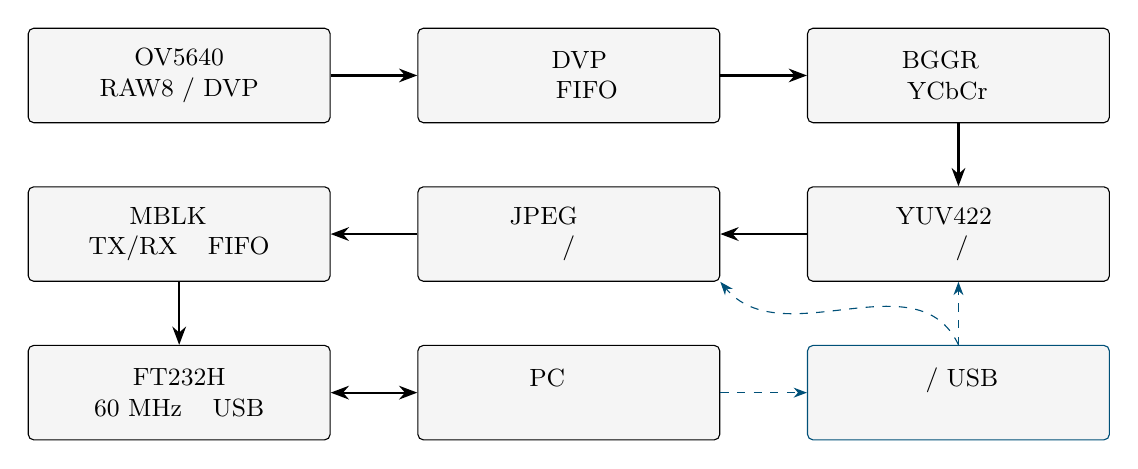
\begin{tikzpicture}[font=\small,>=Stealth,box/.style={draw=navy,fill=shade,rounded corners=2pt,align=center,minimum height=12mm,text width=36mm},node distance=8mm and 11mm]
\node[box] (a) {OV5640\\RAW8 / DVP};
\node[box,right=of a] (b) {引脚寄存与 DVP 捕获\\像素异步 FIFO};
\node[box,right=of b] (c) {BGGR 颜色重建\\YCbCr 降噪};
\node[box,below=of c] (d) {YUV422 预处理\\四模式 / 阈值};
\node[box,left=of d] (e) {JPEG 编码与帧管理\\量化表 / 描述符};
\node[box,left=of e] (f) {MBLK 分块\\TX/RX 异步 FIFO};
\node[box,below=of f] (g) {FT232H\\60 MHz 同步 USB};
\node[box,right=of g] (h) {PC 接收、校验\\独立解码与预览};
\node[box,right=of h,draw=teal] (i) {板载键 / USB 命令\\运行、画质、补光};
\draw[->,thick] (a)--(b);\draw[->,thick] (b)--(c);\draw[->,thick] (c)--(d);\draw[->,thick] (d)--(e);\draw[->,thick] (e)--(f);\draw[->,thick] (f)--(g);\draw[<->,thick] (g)--(h);
\draw[->,teal,dashed] (i)--(d);\draw[->,teal,dashed] (i.north) to[out=115,in=-50] (e.south east);\draw[->,teal,dashed] (h)--(i);
\end{tikzpicture}
\caption{最终系统的流式架构。实线为图像数据通路，虚线为控制关系。}\label{fig:arch}
\end{figure}

\subsection{顶层组织与时钟域}
工程顶层为 \texttt{davinci\_mjpeg\_camera\_top}，帧管理引擎为 \texttt{mjpeg\_camera\_engine}。真实构建选择 \texttt{REAL\_CAMERA=1} 和 profile 5。板上 50 MHz 系统时钟经 MMCM 生成 100 MHz 核心时钟，USB CLKOUT 为 60 MHz；摄像头采样 MMCM 处理外部 PCLK 相位关系。本次实板窗口的 PCLK 计数测得约 75 MHz。

\begin{table}[H]\centering\caption{主要模块的职责边界}
\small\begin{tabularx}{\linewidth}{@{}lY@{}}\toprule
模块组 & 职责\\\midrule
\texttt{rtl/camera} & SCCB、DVP、颜色重建、滤波和预处理\\
\texttt{rtl/core} & 光栅重排、DCT、量化、Zigzag、熵编码和格式化\\
\texttt{rtl/video} & 通道调度、流缓冲、像素接口和载荷归并\\
\texttt{rtl/usb} & 同步总线、跨域 FIFO、状态快照和 MBLK\\
\texttt{rtl/board, top} & 按键与参数、帧生命周期、LED 与 FPS 显示\\\bottomrule
\end{tabularx}\end{table}
源集合由 \texttt{camera\_sources.txt} 维护。模拟 ROM 与渐变源用于回归，真实构建通过常量参数选择输入，综合时移除无效分支。板载 DDR3 保持复位，系统不实例化 MIG 或外部帧存储控制器。
\clearpage

\section{摄像头采集、准入与跨时钟传输}
\subsection{初始化与完整帧准入}
SCCB 控制器完成芯片 ID 读取、寄存器配置和读回，采样时钟就绪后才允许像素路径工作。profile 5 使用 RAW8 BGGR 相位，DVP 捕获模块依据 HREF/VSYNC 和行列计数生成 SOF、EOL、EOF。帧准入同时考虑采样准备、量化表状态、编码忙状态和运行请求。
\lstinputlisting[firstnumber=88,caption={编码引擎的像素握手与帧准入条件},label={lst:admit}]{code/admission.v}
\src{mjpeg/rtl/top/mjpeg_camera_engine.v:88--94}
只有 valid 与 ready 同时有效时，数据及伴随标志才推进。准入请求可在编码开始后降低，已接受的帧由采集模块保持。停止或切换画质时禁止新帧进入，当前帧排完后再转换状态，避免半帧采用新参数。

\subsection{异步 FIFO 与背压}
像素与 USB TX/RX 路径跨越不同时钟域。FIFO 使用二进制地址访问存储器，将灰码指针通过两级同步器送入另一域，并在本地域计算空满。RAM 写口不附加异步复位，便于推断双时钟 BRAM。
\lstinputlisting[firstnumber=15,caption={异步 FIFO 的接受条件、灰码和空满判断},label={lst:fifo}]{code/fifo_gray.v}
\src{mjpeg/rtl/usb/board_test_async_fifo.v:15--21}
灰码减少相邻更新时同时变化的位数，仍需同步器、局部复位释放与物理约束配合。项目同时检查 CDC 和总线偏斜。输出在 \texttt{valid=1, ready=0} 时保持稳定，直到完成握手。

\subsection{异常终止与恢复}
采集模块识别短行、超长行、意外帧界和溢出。故障请求触发 FIFO 清理，核心域产生一次 \texttt{abort}，再通过应答完成恢复；清理结束前不接受下一帧。故障通过失败描述符与计数器报告给主机，避免残余字节拼入后续帧。
\clearpage

\section{颜色重建与空间降噪}
\subsection{RAW8 到 YCbCr 的关系}
RAW8 每个位置只提供 Bayer 阵列中的一个颜色分量。颜色重建依据 BGGR 相位和邻域形成 RGB，再转换到亮度与色度表示。滤波阶段保留 YCbCr444，随后形成 YUV422，使两个水平相邻像素共享一组 Cb/Cr，从而分别处理亮度细节和色度平滑。

3×3 窗口使用行缓存组织，边界采用反射策略。有效位、帧/行标志及参数与数据同步经过流水线；共同使能在背压时暂停各级，保证窗口和元信息始终对应同一像素。系统只需保存局部邻域，缓存规模随图像宽度而非整帧面积增长。

\subsection{中值混合及强度含义}
设窗口中值为 $m$，中心原像素为 $p$，用户强度为 $N\in[0,255]$。中值混合部分使用整数系数
\begin{equation}
a=\min(N,32),\qquad p'=\left\lfloor\frac{32p+a(m-p)+16}{32}\right\rfloor.\label{eq:median}
\end{equation}
$N=0$ 精确保留原像素；8、16、32 对应四分之一、一半和完整中值混合。超过 32 后中值混合系数不再增加，强度继续影响后级亮度引导色度平滑的门限。
\lstinputlisting[firstnumber=70,caption={每个颜色平面的中值混合乘加节选},label={lst:median}]{code/median_mix.v}
\src{mjpeg/rtl/camera/spatial_median_yuv_3x3.v:70--73}
代码把两个加权项改写为“原值加差值乘系数”，每个平面只需一次有符号乘法。三个平面并行，乘加映射至 DSP，以控制 LUT 占用；差值计算单独成级，限制组合路径长度。式\eqref{eq:median}的加 16 对应右移前的舍入项。

\subsection{亮度引导色度平滑}
中值混合后，系统继续对色度执行两级局部平滑，并使用亮度差异限制跨边缘混合，目标是在抑制暗部色斑的同时保留轮廓。较强滤波可能损失纹理，低照度曝光、白平衡和镜头也会影响观感。因此实拍图仅作定性观察，编码载荷下降不能单独证明画质提升。
\clearpage

\section{四模式预处理与参数一致性}
\subsection{模式和数学定义}
彩色模式保留像素；灰度模式将 Cb/Cr 置为 128；二值化将亮度与 $T_b$ 比较；Sobel 依据 3×3 亮度邻域计算梯度。对标准水平、垂直模板计算的 $G_x,G_y$，实现使用绝对值和近似幅值，并归一化到 8 位：
\begin{equation}
E=\min\left(255,\left\lfloor\frac{|G_x|+|G_y|+2}{4}\right\rfloor\right),\quad
Y_{\mathrm{edge}}=\begin{cases}E,&E\geq T_e,\\0,&E<T_e.\end{cases}
\end{equation}
Sobel 保留超过阈值的灰阶边缘幅值，而非把所有有效边缘统一变为白色。其结果需要结合阈值和光照条件解释。
\lstinputlisting[firstnumber=84,caption={四种输出模式的实际 RTL 分支},label={lst:modes}]{code/preprocess_modes.v}
\src{mjpeg/rtl/camera/yuv422_preprocess.v:84--91}

\subsection{配置与像素绑定}
模块把模式、亮度阈值和边缘阈值组合成配置字，随窗口与计算流水线传递。
\texttt{config\_pipe} 与 \texttt{center\_pipe} 对齐，输出采用当前像素对应的配置。参数在帧首锁定；主机同时读取“请求值”与“活动值”，确认设置是否已应用。

\begin{table}[H]\centering\caption{模式、编码和默认行为}
\begin{tabularx}{\linewidth}{@{}lcY@{}}\toprule
模式 & 编码 & 默认行为\\\midrule
彩色 & 00 & 保留 YUV422\\
灰度 & 01 & 保留亮度，Cb/Cr 固定为 128\\
二值化 & 02 & $T_b=128$；亮度达阈值输出 255，否则为 0\\
Sobel & 03 & $T_e=32$；过滤弱边缘，保留梯度强度\\\bottomrule
\end{tabularx}\end{table}
预处理共享有效/就绪流控，在下游暂停时整体保持。灰度、二值化和 Sobel 仍编码为三分量 JPEG；其中性色度使独立解码后的 R、G、B 一致，实板脚本对这一特征进行了检查。
\clearpage

\section{独立 JPEG 编码与帧生命周期}
\subsection{编码步骤与片上缓存}
JPEG 数据通路包含光栅到 MCU 重排、分块 DCT、量化、Zigzag、DC 差分、AC 游程与 Huffman 编码，以及码流标记和字节封装\cite{jpeg}。当前 YUV422 由水平两个亮度块及对应的色度块组成 MCU；局部行组缓存支撑块访问，不使用前一帧作为参考。

二维 DCT 可分解为两个一维变换。对去直流偏置后的 $8\times8$ 样本块 $f$，概念上有
\begin{equation}
F=A f A^{\mathrm T},\qquad \widehat F_{u,v}=\operatorname{round}\!\left(F_{u,v}/Q_{u,v}\right).
\end{equation}
实际 RTL 使用定点常量、流水线和配套量化缩放；是否符合预期由金样比较与独立解码共同检验。量化使用预存值与倒数，通过乘法估计和修正避免通用除法器。Zigzag 将低频系数集中到前部，后续零系数游程与 Huffman 编码形成压缩载荷。

\subsection{画质切换和量化表加载}
系统提供 Q60、Q75、Q85 三组表。运行期间先记录请求；若请求与活动画质不同，禁止接纳新帧，待当前帧结束后加载完整表，再更新活动画质。编码忙期间量化表不可写，避免一个 JPEG 内混合两套 DQT 参数。

\begin{figure}[H]\centering
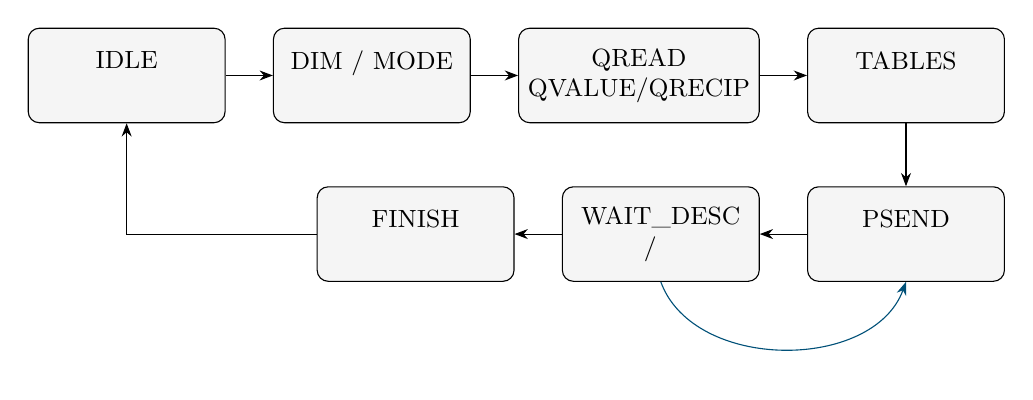
\begin{tikzpicture}[font=\small,>=Stealth,box/.style={draw=navy,rounded corners,fill=shade,align=center,minimum width=25mm,minimum height=12mm},node distance=6mm]
\node[box] (a) {IDLE\\等待运行};\node[box,right=of a] (b) {DIM / MODE\\尺寸与模式};\node[box,right=of b] (c) {QREAD\\QVALUE/QRECIP};\node[box,right=of c] (d) {TABLES\\等待表就绪};
\node[box,below=8mm of d] (e) {PSEND\\像素流};\node[box,left=of e] (f) {WAIT\_DESC\\完成/失败描述符};\node[box,left=of f] (g) {FINISH\\排完并结束};
\draw[->] (a)--(b);\draw[->] (b)--(c);\draw[->] (c)--(d);\draw[->] (d)--(e);\draw[->] (e)--(f);\draw[->] (f)--(g);\draw[->] (g.west)-| (a.south);\draw[->,teal] (f.south) to[out=-70,in=-110] node[below]{继续运行} (e.south);
\end{tikzpicture}
\caption{引擎主要状态关系。实际转移还受握手、停止请求和描述符约束。}
\end{figure}

\subsection{描述符与停止语义}
成功和失败均通过描述符结束帧生命周期。\texttt{success\_frame} 和 \texttt{failed\_frame} 来自已接受的最终描述符，不能只统计输入 SOF。停止命令先排完正在处理的帧及输出记录，再发送 END，使主机判断会话是否完整闭合，并区分输入、成功与失败计数。
\clearpage

\section{同步 USB、MBLK 与板卡控制}
\subsection{同步总线和分块传输}
USB 域采用 FT232H 的 60 MHz CLKOUT。写方向的数据、WR\# 与三态输出经过寄存，接受时刻由 TXE\# 与写选通共同判定；读方向通过 RELEASE、OE\_SETUP、READ、TURN 完成总线换向，避免双方同时驱动。两字节弹性前端保存阻塞期间的预取数据，晚到的 TXE\# 不直接进入宽 FIFO 的出队反馈路径。

MBLK 具有 8 字节头部：4 字节标识、kind、flags 与 16 位 body 长度，整数按小端编码。数据块含帧号及至多 1024 字节 JPEG；描述符、FPS、时序、链路和摄像头状态分别发送。描述符包含帧号、64 位时间戳、载荷长度、尺寸及错误状态。归并载荷可降低细粒度封包开销，同时保留完整帧边界。

\begin{table}[H]\centering\caption{主机控制接口节选}
\small\begin{tabularx}{\linewidth}{@{}lYlY@{}}\toprule
命令 & 功能 & 命令 & 功能\\\midrule
\texttt{C / S} & 启动 / 排完后停止 & \texttt{1/2/3} & Q60 / Q75 / Q85\\
\texttt{L / l} & 两秒补光 / 关闭 & \texttt{Nxx} & 降噪强度 00～FF\\
\texttt{Bxx} & 二值化阈值 & \texttt{Exx} & Sobel 阈值\\
\texttt{Mxx} & 00～03 四模式 & 换行 & 提交多字节设置\\\bottomrule
\end{tabularx}\end{table}

\subsection{原子命令与停止优先级}
载荷中可能出现十六进制 C/F，畸形输入也可能含 S/L。解析器隔离载荷期间的单字节控制，等换行后统一提交；板载按键仍可响应。
\lstinputlisting[firstnumber=97,caption={设置命令在换行处原子提交},label={lst:atomic}]{code/atomic_config.v}
\src{mjpeg/rtl/board/camera_board_controls.v:97--108}
KEY0 启停、KEY1 切换画质、KEY2 请求补光、KEY3 停止并关灯；同时操作时停止优先。补光定时由 FPGA 管理，PC 停顿不会延长请求的照明时间；LED 与数码管反映运行、画质、灯光和压缩 FPS。
\clearpage

\section{上位机与工程精简}
\subsection{接收、独立解码与显示}
Python 接收器经 D2XX 打开数据芯片，只修改易失 FIFO 模式，不重写 EEPROM。\texttt{block\_records.py} 检查包长、顺序、JPEG 边界及载荷与描述符一致性；严格接收器进一步检查尺寸、帧号和时间戳。Pillow 对成功帧执行完整解压，避免仅凭文件头或 SOI/EOI 判断成功。
\lstinputlisting[language=Python,firstnumber=52,caption={严格接收器的完整 JPEG 解码节选},label={lst:decode}]{code/jpeg_decode.py}
\src{mjpeg/host/camera_receiver.py:52--61}
查看器将解码与缩放放在后台，预览队列只保留最新帧，避免刷新阻塞 USB。预览跳过与板卡采集丢帧分别统计：前者反映主机调度，后者须结合准入和溢出计数解释。

\subsection{精简范围和保留原则}
工程删除了退出最终链路的 DDR3/MIG 归档、参考块复用、自适应系数阈值、首版 RGB 降噪、UART 和旧板卡顶层，以及过期报告、接口和跨层参数。独立提取摄像头引擎，统一源清单、GUI 工程、构建和编程入口。清理记录共移除 3576 个 Git 跟踪的历史文件，保留 72 个最终功能基线证据文件。

内部确定存在的属性和固定配置可直接使用；外部数据完整性、CDC、FIFO 背压、时序约束和异常恢复仍属于功能要求。项目保留这些机制，以维持对真实链路行为的可观察性。

\subsection{验收脚本的一次残留问题}
上板时发现降噪脚本仍发送已删除的 T/A 旧命令，其载荷中的 F 被既有单字节兼容命令解释为启动，导致“等待停止”超时。修正移除旧探测，保留当前 N 命令畸形载荷隔离检查。七段重测和 59 项 Python 测试随后通过，汇总保留首轮失败与重测，说明精简需同步维护测试和主机工具。
\clearpage

\section{仿真方案与原生波形分析}
\subsection{分层验证和覆盖范围}
验证采用软件参考、RTL 模块、链路集成和板卡验收四个层次。2026 年 10 月 9 日完成 59 项 Python 测试和表\ref{tab:sim}的 7 项 RTL 回归，并对 6 个板卡控制场景及 3 个摄像头场景的 JPEG 执行逐字节金样比较。同步 USB 集成仿真验证了 18 帧。

\begin{table}[H]\centering\caption{RTL 回归测试及主要覆盖项}\label{tab:sim}
\small\begin{tabularx}{\linewidth}{@{}p{61mm}Y@{}}\toprule
测试平台 & 覆盖内容\\\midrule
\nolinkurl{tb_camera_board_controls} & 去抖、长按单次触发、停止优先、原子提交及解析超时\\
\nolinkurl{tb_mjpeg_board_controls} & 画质表切换、帧生命周期、控制与编码协同\\
\nolinkurl{tb_mjpeg_real_camera} & DVP、像素 CDC、编码、MBLK、短行 abort 及恢复\\
\nolinkurl{tb_mjpeg_payload_coalescer} & 载荷归并、有效字节数、包结束\\
\nolinkurl{tb_mjpeg_block_transport} & 分块、描述符和状态复用\\
\nolinkurl{tb_board_test_async_fifo} & 异步读写、满队列、回绕、停钟和数据保持\\
\nolinkurl{tb_davinci_mjpeg_sync_test} & 同步 FT245 总线与完整 JPEG 输出集成\\\bottomrule
\end{tabularx}\end{table}

\subsection{本次波形导出的范围}
2026 年 10 月 25 日补跑板卡控制和摄像头链路两项测试，启用调试可见性并导出 VCD/WDB，随后使用 Vivado 2020.1 原生窗口截图。WDB 保存波形活动，WCFG 保存信号、时间范围和列宽等显示配置\cite{ug900}。正文裁取原生波形区域以保证字号可读，完整窗口 PNG 和数据库仍保留在工程附件中。

摄像头测试使用 $48\times16$ 的 YUYV 激励，核心时钟周期 10 ns、PCLK 周期 40 ns，并随机拉低输出 ready。它检验采集、CDC、JPEG 与封包的集成关系，不直接复现生产链路 RAW8 颜色重建、1080p 尺寸及所有模拟器件行为。后者需要结合对应软件参考和实板结果判断。

软件测试覆盖当前图像参考、主机协议和控制行为，独立 JPEG 金样提供字节级确定性验证；实拍图像不能与固定金样逐字节比较，应检查格式、连续性、错误状态、尺寸与完整解码。分层判定有助于区分算法错误、封包错误和器件连接问题。
\evid{mjpeg/docs/精简验证.json；waveforms_20261025/waveform_summary.json}
\clearpage

\subsection{摄像头完整帧、故障与恢复}
\begin{figure}[H]\centering
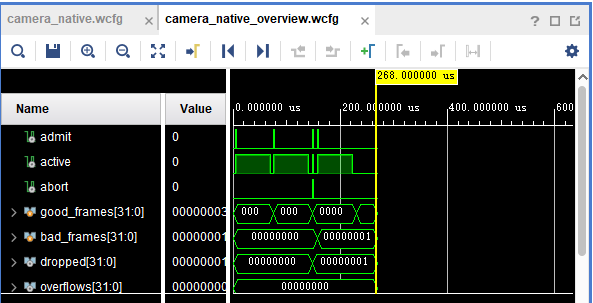
\includegraphics[width=.86\linewidth]{native_camera_crop.png}
\caption{Vivado 原生摄像头链路波形区域。最终成功 3、失败 1、丢弃 1、溢出 0；总线值沿用原生窗口基数。}\label{fig:simcamera}
\end{figure}
图\ref{fig:simcamera}中，\texttt{admit} 允许新帧进入，\texttt{active} 覆盖接收区间。测试在第三次尝试中仅发送 13 个像素构造短行，触发一次 \texttt{abort}，失败与丢弃计数各增一次；随后完整帧再次成功，最终 \texttt{good\_frames=3}。该失败是预期测试事件，不代表正常输入下的随机丢帧。

\begin{figure}[H]\centering
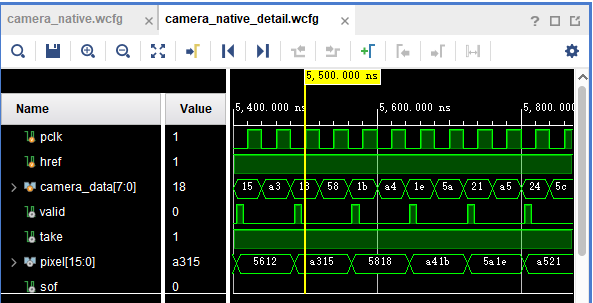
\includegraphics[width=.86\linewidth]{native_pixels_crop.png}
\caption{Vivado 原生像素握手细节，约 5.4～5.8 $\mu$s；光标为 5500 ns。}\label{fig:simpixel}
\end{figure}
图\ref{fig:simpixel}显示 PCLK、HREF 和 8 位输入字节，捕获后形成 16 位 YUV422 像素。\texttt{valid} 与 \texttt{take} 共同决定接受时刻；总线上的保持区间不代表重复接受。SOF/EOL/EOF 仅在像素 valid 有效时具有语义，分析时须同时观察握手。
\evid{camera.wdb；vivado_camera_overview.png；vivado_pixel_handshake.png}
\clearpage

\subsection{板卡控制波形和测试激励}
\begin{figure}[H]\centering
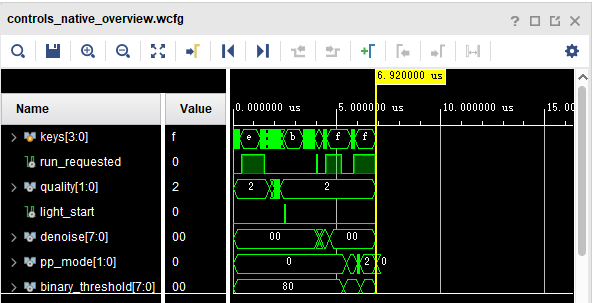
\includegraphics[width=.93\linewidth]{native_controls_crop.png}
\caption{Vivado 原生控制波形：按键、运行请求、画质、降噪强度与模式设置。}\label{fig:simcontrols}
\end{figure}
图\ref{fig:simcontrols}中按键低有效。测试构造抖动、长按、单次按键和 USB 字节，检查运行请求不会由接点抖动反复翻转。\texttt{quality} 的内部编码 0/1/2 对应 Q60/Q75/Q85。降噪和模式设置在完整命令结束时改变，非法模式和畸形载荷不能提交或泄漏为启停、补光。

代码\ref{lst:test}列出摄像头仿真的主要激励：前两帧正常，第三次发送短行，之后发送含帧中 STOP 的完整帧并等待输出。
\lstinputlisting[language=Verilog,firstnumber=86,caption={摄像头测试中的故障注入和恢复检查},label={lst:test}]{code/sim_fault_recovery.sv}
\src{mjpeg/tb/tb_mjpeg_real_camera.sv:86--92}

\subsection{通过判定和复核}
测试平台通过断言和最终 PASS 标记检查结果。工具正常退出不足以替代断言检查，脚本还检索 \texttt{Fatal:} 和目标标记。摄像头场景必须同时满足 3 帧成功、1 次失败、1 次 abort、3 帧接收、1 次丢弃和 0 次溢出。完整 VCD 可进一步放大脉冲，WDB/WCFG 可恢复原生显示。
\evid{BUTTON_DEBOUNCE_PASS.txt；REAL_CAMERA_SIM_PASS.txt；simulation.log}
\clearpage

\section{综合实现、资源与时序}
\subsection{当前固件的实现后结果}
2026 年 10 月 11 日从精简源码重新执行综合、布局布线及 bitstream 生成，构建目录为 \texttt{full\_20261011\_123231}。表\ref{tab:resource}采用实现后数据，避免把早期综合估算与最终资源混用。

\begin{table}[H]\centering\caption{当前固件的实现后资源占用}\label{tab:resource}
\begin{tabular}{@{}lrrr@{}}\toprule
资源 & 已使用 & 可用 & 占用率\\\midrule
Slice LUT & 15544 & 20800 & 74.73\%\\
Slice Register & 19523 & 41600 & 46.93\%\\
Block RAM Tile & 36 & 50 & 72.00\%\\
DSP48E1 & 46 & 90 & 51.11\%\\
Bonded IOB & 55 & 250 & 22.00\%\\\bottomrule
\end{tabular}\end{table}
LUT 低于项目设定的 80\% 上限。BRAM 服务于行组缓存、空间窗口、码流与跨域 FIFO。系统使用片上缓存保持流式访问，当前资源余量仍约束后续扩展。

\begin{table}[H]\centering\caption{最终静态时序及构建检查}
\begin{tabularx}{\linewidth}{@{}lY@{}}\toprule
项目 & 结果及解释\\\midrule
最差建立裕量 & WNS $+0.050$ ns；TNS 为 0，失败端点为 0\\
最差保持裕量 & WHS $+0.015$ ns；THS 为 0，失败端点为 0\\
核心时钟域 & 100 MHz core\_raw 域 WNS 为 $+0.440$ ns\\
USB 时钟域 & usb\_clk 域 WNS 为 $+0.064$ ns\\
构建检查 & CDC、总线偏斜、DRC 错误、黑盒及 USB 三态释放检查通过\\
下载检查 & CRC 正常，DONE/EOS 置位，生成 PROGRAM\_PASS\\\bottomrule
\end{tabularx}\end{table}

\subsection{结果含义与剩余风险}
最差建立路径跨越外部摄像头输入与采样时钟，正裕量较小；USB 保持裕量也偏小。结果表示满足本次约束与实现条件，不能推断修改引脚、器件或约束后仍有相同余量。DRC 无错误仍保留警告，涉及摄像头非专用时钟布线、RAM 异步控制等，需要结合硬件和复位语义继续审查。一次通过不代表所有温压条件与板间差异均已覆盖。

\evid{full_20261011_123231/utilization.rpt；timing_routed.rpt；BUILD_PASS.txt；PROGRAM_PASS.txt}
\clearpage

\section{实板运行与验收}
\subsection{测试条件与验收组成}
测试使用达芬奇 XC7A35T、OV5640 和 FT232H。经 JTAG 下载重新构建的固件，检查芯片 ID 为 \texttt{0x5640} 和初始化状态，再通过 D2XX 独占数据接口采集。分辨率为 $1920\times1080$、画质默认 Q85、核心域 100 MHz；各阶段改变模式、滤波与运行状态，结束后停止并关灯。

\begin{table}[H]\centering\caption{2026-10-11 实板验收组成}
\begin{tabularx}{\linewidth}{@{}l r Y@{}}\toprule
阶段 & 解码帧数 & 主要覆盖项\\\midrule
板卡控制 & 690 & 三档画质、两次启停、补光限时读回\\
预处理轮换 & 811 & 四模式及多个亮度/边缘阈值\\
降噪重测 & 840 & 0、8、16、32、64、255、0 七段切换\\
降噪与模式组合 & 180 & N32 下 Sobel 与彩色配合\\
连续彩色 & 1795 & 60 s，N32；严格检查帧率和稳态丢帧\\
连续 Sobel / 彩色 & 3600 & 各 60 s，N0；各 1800 帧\\\midrule
主体功能验收 & 7916 & 以上六阶段合计\\
查看器收流 & 117 & 自动启动、完整解码、正常退出\\\midrule
总计 & 8033 & 各阶段全部通过\\\bottomrule
\end{tabularx}\end{table}

\subsection{持续运行与计数解释}
严格彩色长测得到 30.0019328 fps。输入与压缩窗口统计为 30 fps，59 个有效状态间隔内接收 1770 帧，\texttt{dropped\_frames} 和 \texttt{overflow\_count} 增量均为 0；成功 JPEG 序号 0～1794。1795 帧包含启动和停止时刻的影响，应采用实际接收帧数，不能直接以 $60\times30$ 替代。

查看器及空闲期间可能出现准入跳过，因为停止或准备参数时系统有意拒绝传感器帧。判断链路故障应结合稳定窗口差值和溢出状态，不能把累计 dropped 非零全部理解为传输错误。

\subsection{交互验证边界}
补光已观察到“开启”和定时“关闭”的寄存器读回。软件控制、按键逻辑仿真和最终停止状态均通过；实板按钮手感、实际灯光亮灭外观尚未由人工确认，保留为待完成的物理观察项。
\evid{cleanup_acceptance_20261011_124020/hardware_summary.json}
\clearpage

\subsection{本次演示采集条件与读图方法}
2026 年 10 月 26 日从正在使用的 \texttt{camera\_viewer.py} 实时演示窗口补充采集。摄像头对准实验室置物架、桌椅、纸箱及设备，维持视角和照明环境，按顺序切换板内模式和参数。所有截图均来自真实运行窗口，包含预处理按钮、阈值输入框、图像与底部状态栏；没有用 PC 算法生成灰度、二值化或边缘效果。

本次固定分辨率 $1920\times1080$、降噪强度 N32。模式与阈值对比固定 Q85；画质对比固定彩色、亮度阈值 128、边缘阈值 18。每次提交后至少等待 3 s，并确认板卡返回的实际设置与目标一致，再记录稳定窗口。模式和阈值各记录约 8 s，画质各记录约 12 s；原始采样长度、逐帧大小、板卡时间戳、状态读回和截图一并保存。

\begin{table}[H]\centering\caption{本次演示截图覆盖范围}\label{tab:livecoverage}
\small\begin{tabularx}{\linewidth}{@{}p{29mm}p{57mm}Y@{}}\toprule
类别 & 采集设置 & 固定条件\\\midrule
基础模式 & 彩色、灰度、二值化、Sobel & 1080p，N32，Q85\\
二值化阈值 & $T_b=64,96,128,160,192,224$ & 边缘阈值 18，Q85\\
边缘阈值 & $T_e=8,18,32,64$ & 亮度阈值 128，Q85\\
JPEG 画质 & Q60、Q75、Q85，末尾重复 Q60 & 彩色，N32，1080p\\\bottomrule
\end{tabularx}\end{table}

底部“JPEG fps”依据接收帧的 FPGA 时间戳统计；“显示 fps”受主机解码、缩放和窗口刷新影响。预览队列仅保留最新帧，所以“预览跳过”不等价于硬件丢帧。判断板卡链路需检查板内输入/压缩/失败 fps、编码失败、溢出和稳定窗口丢帧增量。截图中的累计准入跳帧还包含停止、启动等历史阶段，不能直接当作当前采样窗口的故障。

后续图注的带宽为独立稳定窗口平均值，截图底部是约 1 s 的即时刷新值，两者存在小幅差别。截图只改变排版尺寸，完整原图随工程提供。各参数分时采集；自动曝光、白平衡与室内光源波动未锁定，因此适合说明功能与本场景带宽变化，不能作为严格的同输入画质评价。
\evid{evidence/live_demo_summary.json；evidence/*_t*.json；images/*_window.png}
\clearpage
\subsection{彩色与灰度模式}
\begin{figure}[H]\centering
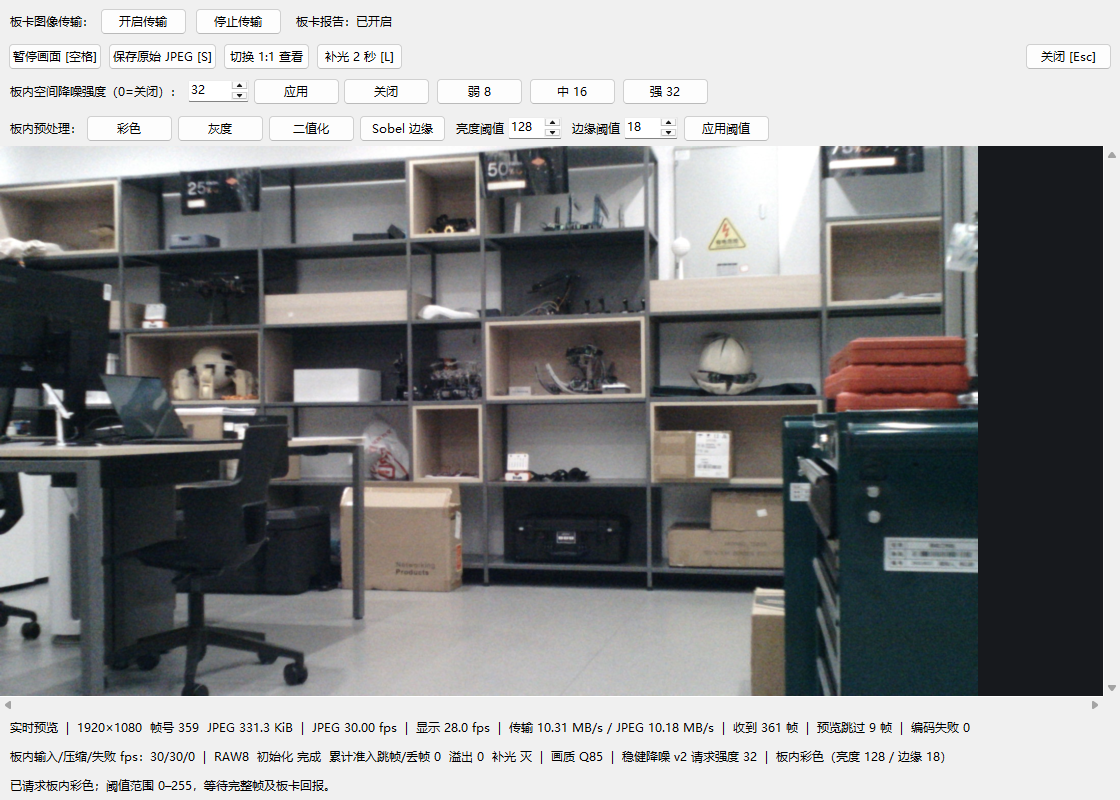
\includegraphics[width=.82\linewidth]{mode_color_window.png}
\caption{彩色模式，Q85，N32。置物架、设备和地面的颜色与亮度层次均可辨认。截图时 JPEG 331.3 KiB；稳定窗口 JPEG 载荷 10.15 MB/s、USB 接收 10.27 MB/s。}\label{fig:live-color}
\end{figure}
\begin{figure}[H]\centering
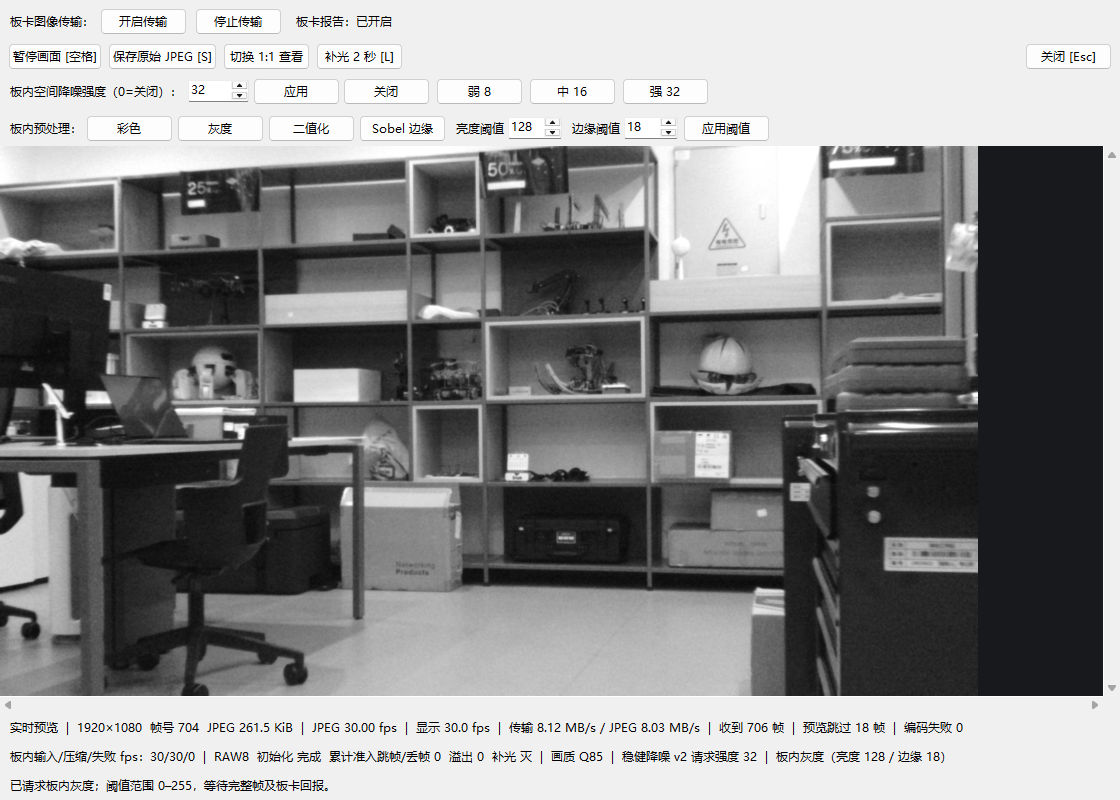
\includegraphics[width=.82\linewidth]{mode_gray_window.png}
\caption{灰度模式，Q85，N32。场景空间结构保留，色彩信息转为亮度层次。截图时 JPEG 261.5 KiB；稳定窗口 JPEG 载荷 8.05 MB/s、USB 接收 8.15 MB/s。}\label{fig:live-gray}
\end{figure}
\clearpage
\subsection{二值化阈值对比的判读}
二值化在板内比较像素亮度与阈值：$Y_{\rm out}=255$ 当 $Y\geq T_b$，否则输出 0，并将色度置为中性。提高 $T_b$ 后，只有更亮的区域保留为白色。本次选取 64～224 的六档设置，以覆盖大面积亮区、主要物体分割及高亮区域筛选。

以下各页分别显示两档真实窗口。低阈值下置物架、地面等大面积区域可能连成白块；阈值升高时较暗的隔板、设备和背景逐渐转黑，高阈值主要保留强亮区。JPEG 为有损编码，二值边界在解码后可能出现灰色过渡或轻微振铃，不能只据此判断 FPGA 比较逻辑错误。

\begin{table}[H]\centering\caption{二值化各阈值的实测载荷}\label{tab:binaryrates}
\small\begin{tabular}{@{}rrrrr@{}}\toprule
$T_b$ & 样本帧数 & 平均 JPEG (kB) & JPEG (MB/s) & USB 接收 (MB/s)\\\midrule
64 & 244 & 262.95 & 7.897 & 7.992\\
96 & 242 & 279.41 & 8.387 & 8.488\\
128 & 241 & 230.25 & 6.910 & 7.000\\
160 & 242 & 166.14 & 4.977 & 5.038\\
192 & 244 & 144.63 & 4.353 & 4.406\\
224 & 244 & 83.89 & 2.519 & 2.551\\
\bottomrule\end{tabular}\end{table}
白色面积不是码率的唯一决定因素；边界数量、形状和图像高频成分也会影响 JPEG 大小。中间阈值可能产生较复杂的明暗分界，载荷不要求随阈值单调变化。
\clearpage
\subsection{二值化阈值 64 与 96}
\begin{figure}[H]\centering
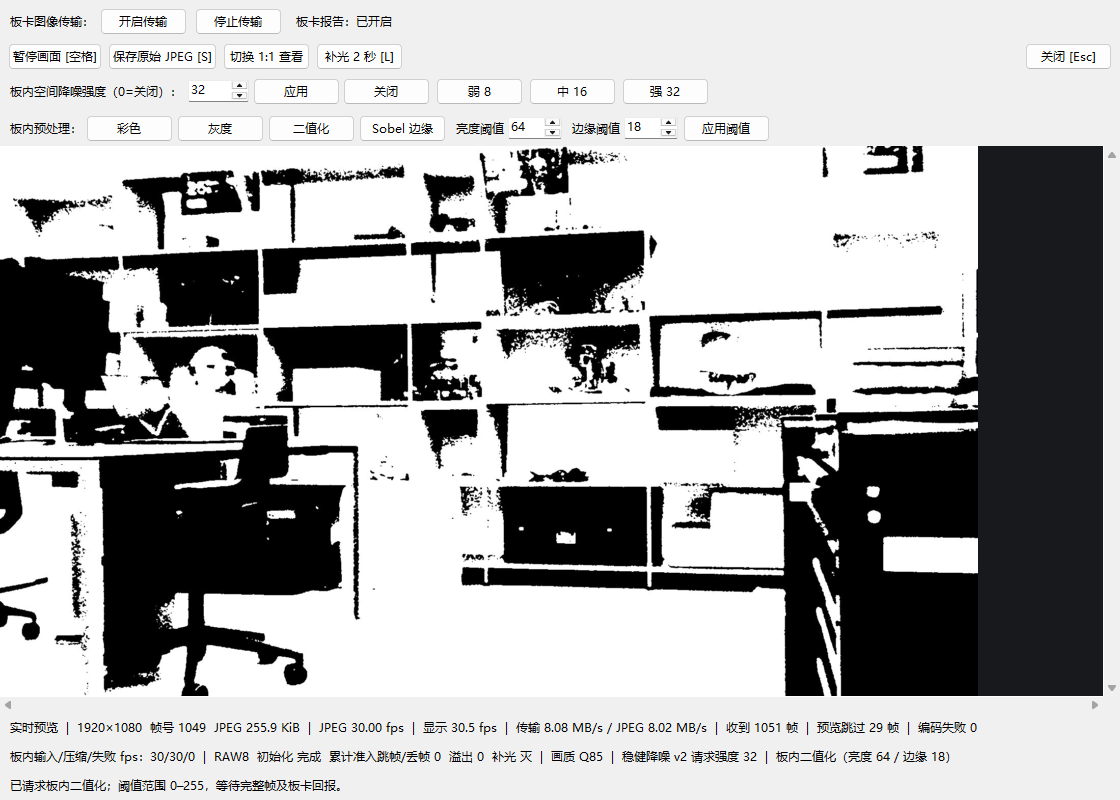
\includegraphics[width=.82\linewidth]{binary_t064_window.png}
\caption{二值化，$T_b=64$，Q85，N32。截图时 JPEG 255.9 KiB；稳定窗口 JPEG 载荷 7.90 MB/s、USB 接收 7.99 MB/s。}\label{fig:binary-64}
\end{figure}
\begin{figure}[H]\centering
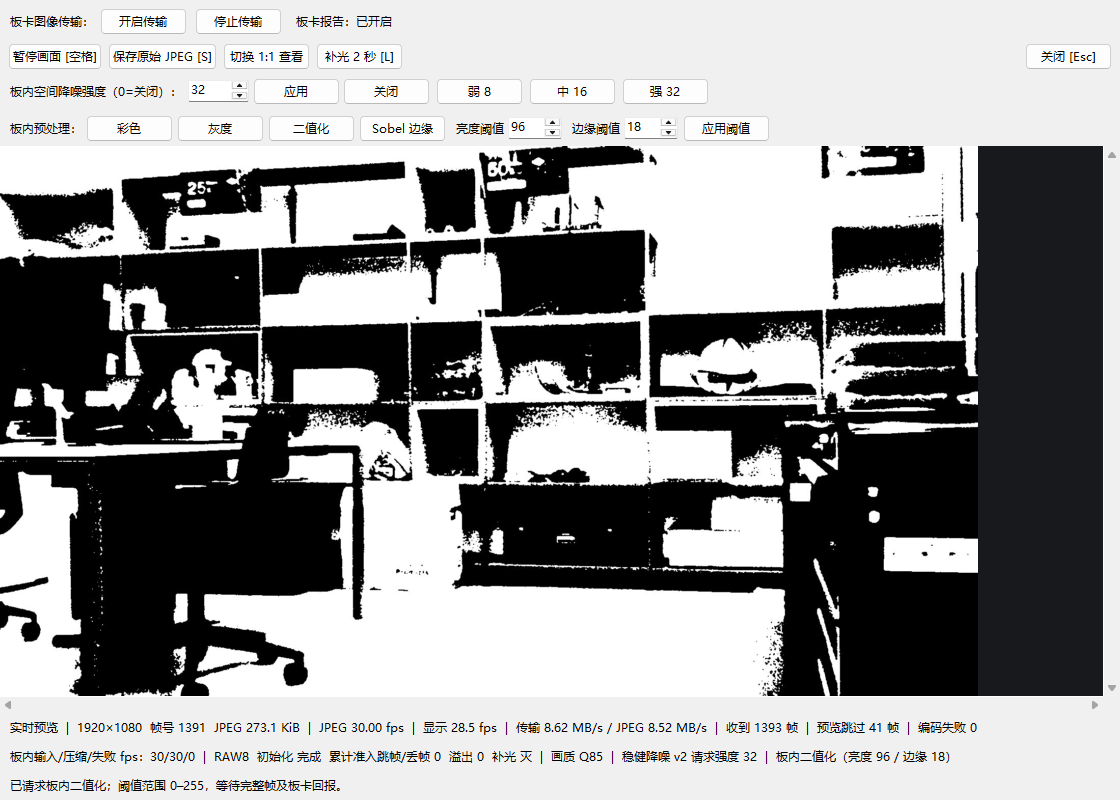
\includegraphics[width=.82\linewidth]{binary_t096_window.png}
\caption{二值化，$T_b=96$，Q85，N32。截图时 JPEG 273.1 KiB；稳定窗口 JPEG 载荷 8.39 MB/s、USB 接收 8.49 MB/s。}\label{fig:binary-96}
\end{figure}
\clearpage
\subsection{二值化阈值 128 与 160}
\begin{figure}[H]\centering
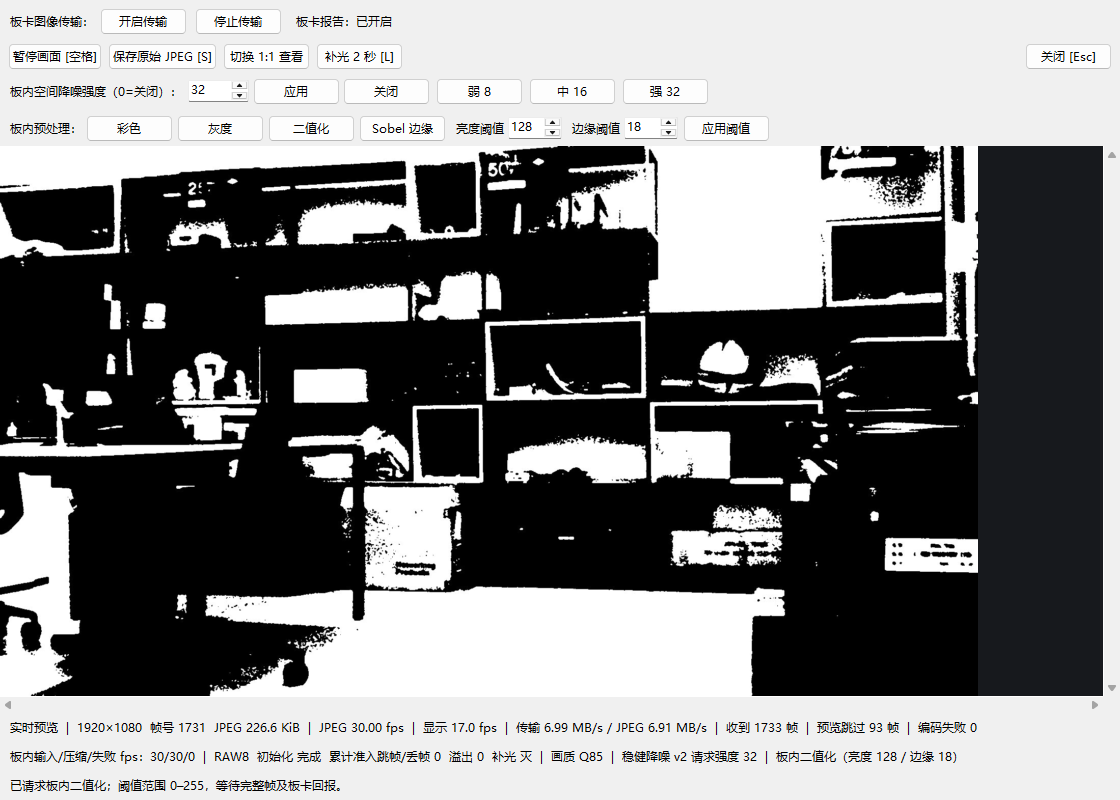
\includegraphics[width=.82\linewidth]{binary_t128_window.png}
\caption{二值化，$T_b=128$，Q85，N32。截图时 JPEG 226.6 KiB；稳定窗口 JPEG 载荷 6.91 MB/s、USB 接收 7.00 MB/s。}\label{fig:binary-128}
\end{figure}
\begin{figure}[H]\centering
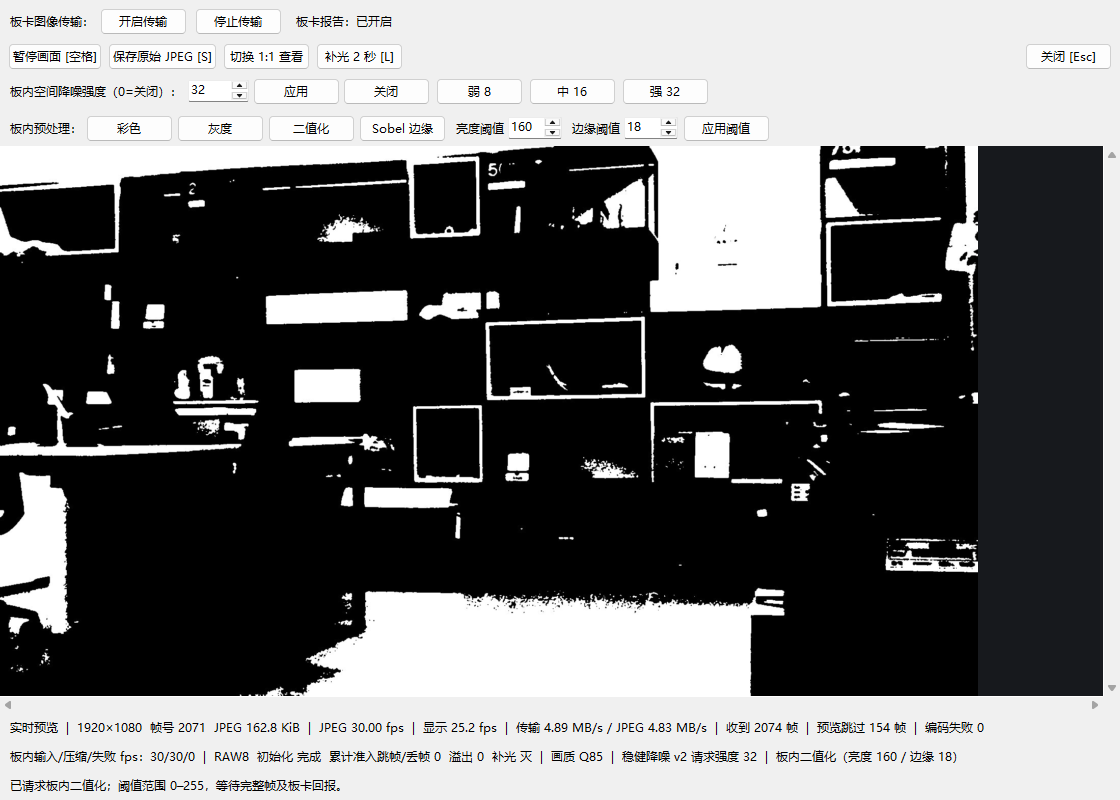
\includegraphics[width=.82\linewidth]{binary_t160_window.png}
\caption{二值化，$T_b=160$，Q85，N32。截图时 JPEG 162.8 KiB；稳定窗口 JPEG 载荷 4.98 MB/s、USB 接收 5.04 MB/s。}\label{fig:binary-160}
\end{figure}
\clearpage
\subsection{二值化阈值 192 与 224}
\begin{figure}[H]\centering
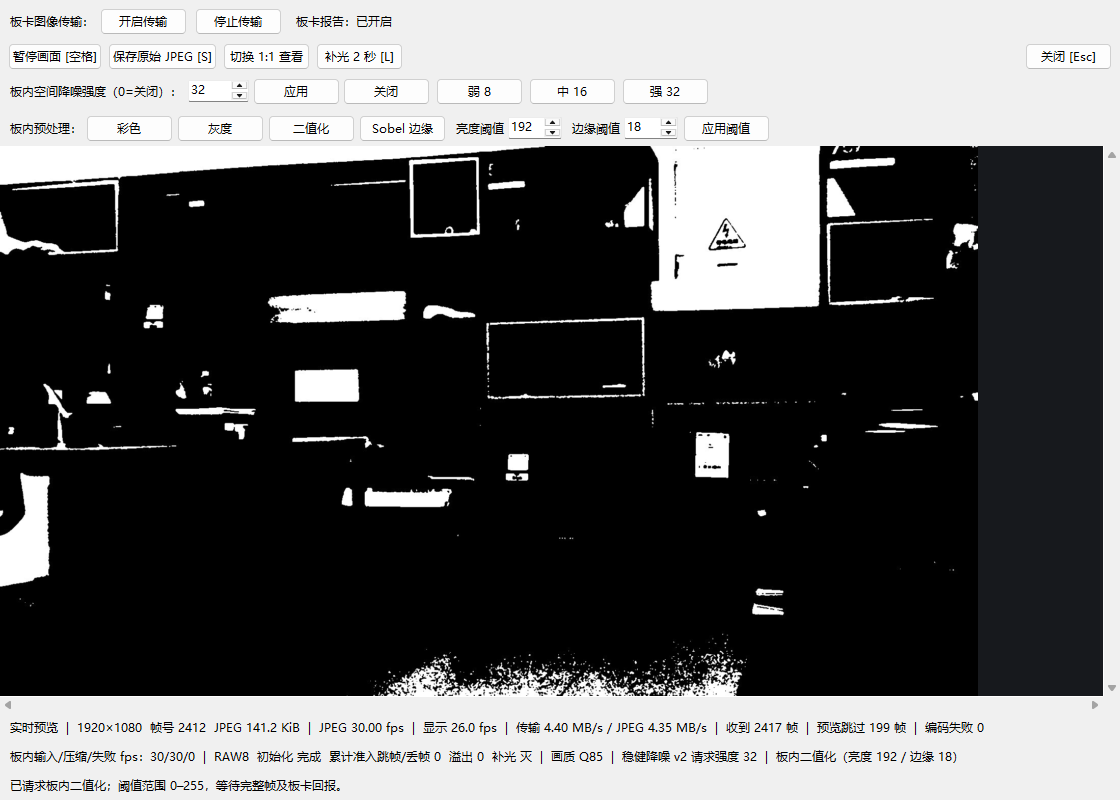
\includegraphics[width=.82\linewidth]{binary_t192_window.png}
\caption{二值化，$T_b=192$，Q85，N32。截图时 JPEG 141.2 KiB；稳定窗口 JPEG 载荷 4.35 MB/s、USB 接收 4.41 MB/s。}\label{fig:binary-192}
\end{figure}
\begin{figure}[H]\centering
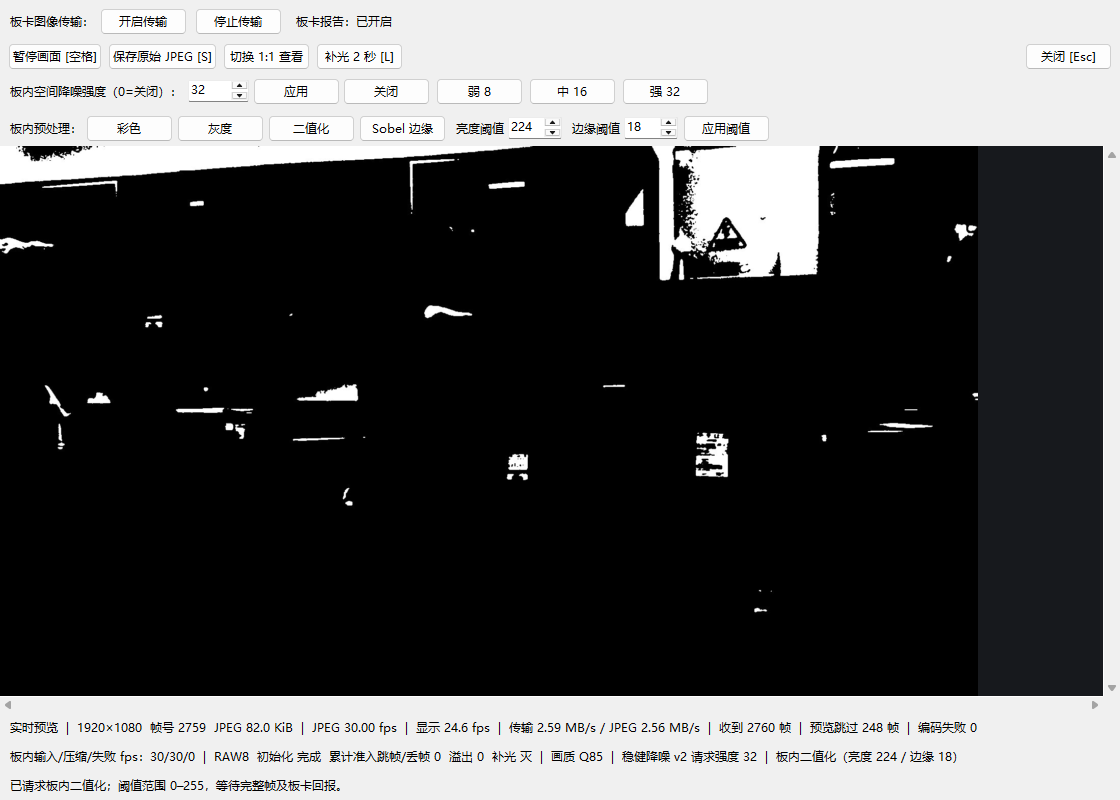
\includegraphics[width=.82\linewidth]{binary_t224_window.png}
\caption{二值化，$T_b=224$，Q85，N32。截图时 JPEG 82.0 KiB；稳定窗口 JPEG 载荷 2.52 MB/s、USB 接收 2.55 MB/s。}\label{fig:binary-224}
\end{figure}
\clearpage
\subsection{Sobel 阈值对比的判读}
当前 RTL 计算 $G_x$ 与 $G_y$ 后，使用
\[
 E=\min\!\left(255,\left\lfloor\frac{|G_x|+|G_y|+2}{4}\right\rfloor\right),
 \qquad Y_{\rm out}=\begin{cases}E,&E\geq T_e,\\0,&E<T_e.\end{cases}
\]
边缘模式保留超过阈值的梯度幅度，并不把每个边缘像素放大成纯白色。因此截图中的轮廓呈不同亮度，高阈值画面变暗也是符合实现的结果。

$T_e=8$ 能显示较多隔板、椅背、纸箱及细小纹理，但也容易保留弱变化；提高到 18、32 后，弱边缘减少；64 主要留下较强的亮度跃迁，部分连续轮廓会变细或中断。阈值应结合实际照度和目标边缘强度选择，不能只凭图像亮度高低判断检测质量。

\begin{table}[H]\centering\caption{Sobel 各阈值的实测载荷}\label{tab:edgerates}
\small\begin{tabular}{@{}rrrrr@{}}\toprule
$T_e$ & 样本帧数 & 平均 JPEG (kB) & JPEG (MB/s) & USB 接收 (MB/s)\\\midrule
8 & 240 & 293.20 & 8.778 & 8.884\\
18 & 243 & 200.69 & 6.037 & 6.101\\
32 & 244 & 173.00 & 5.184 & 5.247\\
64 & 240 & 93.24 & 2.797 & 2.832\\
\bottomrule\end{tabular}\end{table}
\src{mjpeg/rtl/camera/yuv422_preprocess.v}
\clearpage
\subsection{Sobel 边缘阈值 8 与 18}
\begin{figure}[H]\centering
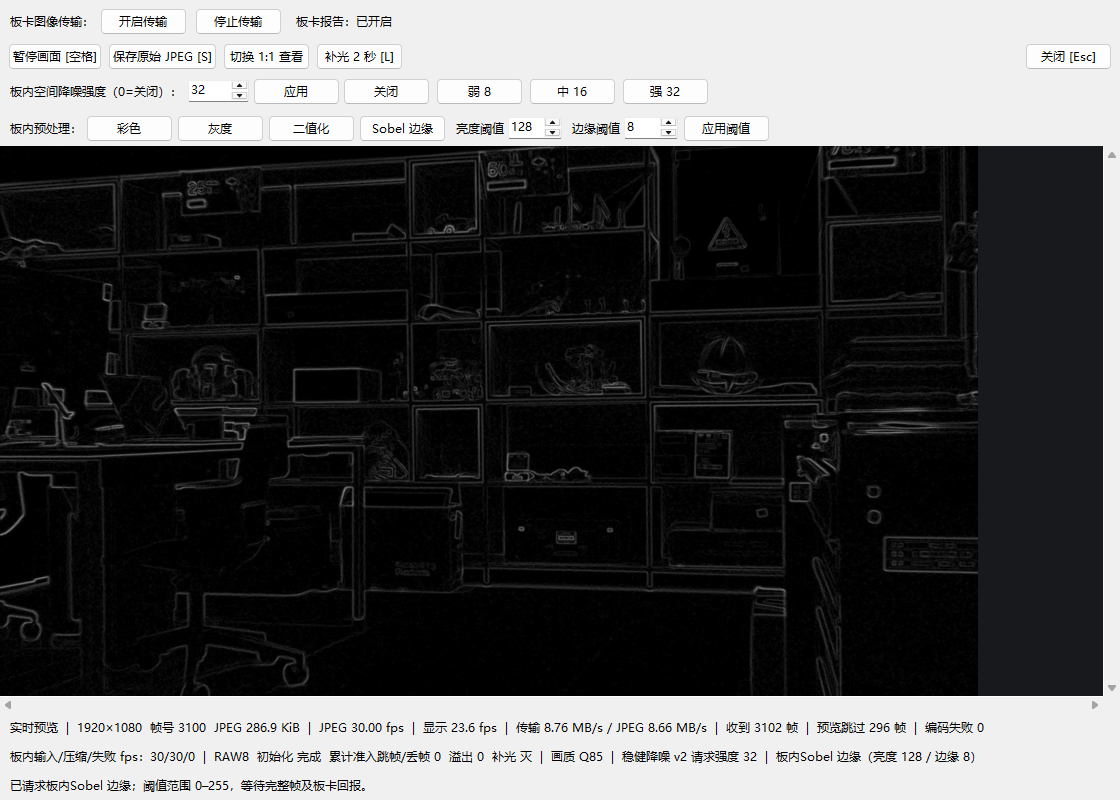
\includegraphics[width=.82\linewidth]{sobel_t008_window.png}
\caption{Sobel 边缘，$T_e=8$，Q85，N32。截图时 JPEG 286.9 KiB；稳定窗口 JPEG 载荷 8.78 MB/s、USB 接收 8.88 MB/s。}\label{fig:edge-8}
\end{figure}
\begin{figure}[H]\centering
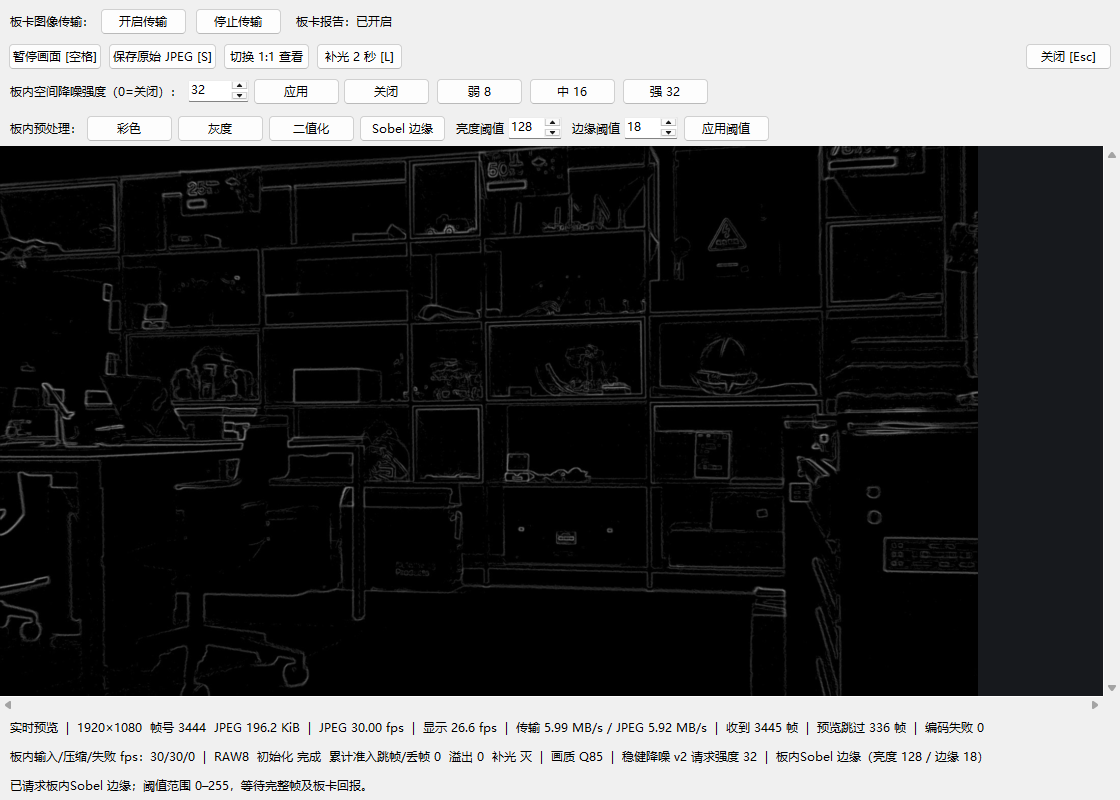
\includegraphics[width=.82\linewidth]{sobel_t018_window.png}
\caption{Sobel 边缘，$T_e=18$，Q85，N32。截图时 JPEG 196.2 KiB；稳定窗口 JPEG 载荷 6.04 MB/s、USB 接收 6.10 MB/s。}\label{fig:edge-18}
\end{figure}
\clearpage
\subsection{Sobel 边缘阈值 32 与 64}
\begin{figure}[H]\centering
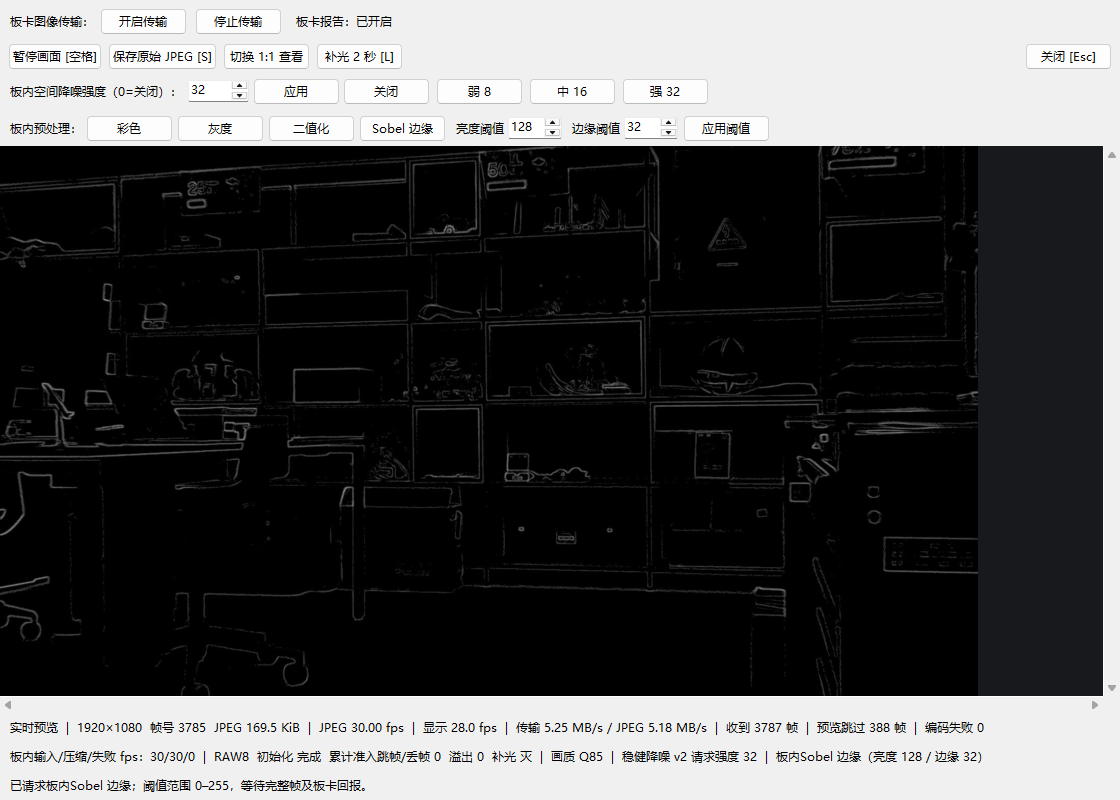
\includegraphics[width=.82\linewidth]{sobel_t032_window.png}
\caption{Sobel 边缘，$T_e=32$，Q85，N32。截图时 JPEG 169.5 KiB；稳定窗口 JPEG 载荷 5.18 MB/s、USB 接收 5.25 MB/s。}\label{fig:edge-32}
\end{figure}
\begin{figure}[H]\centering
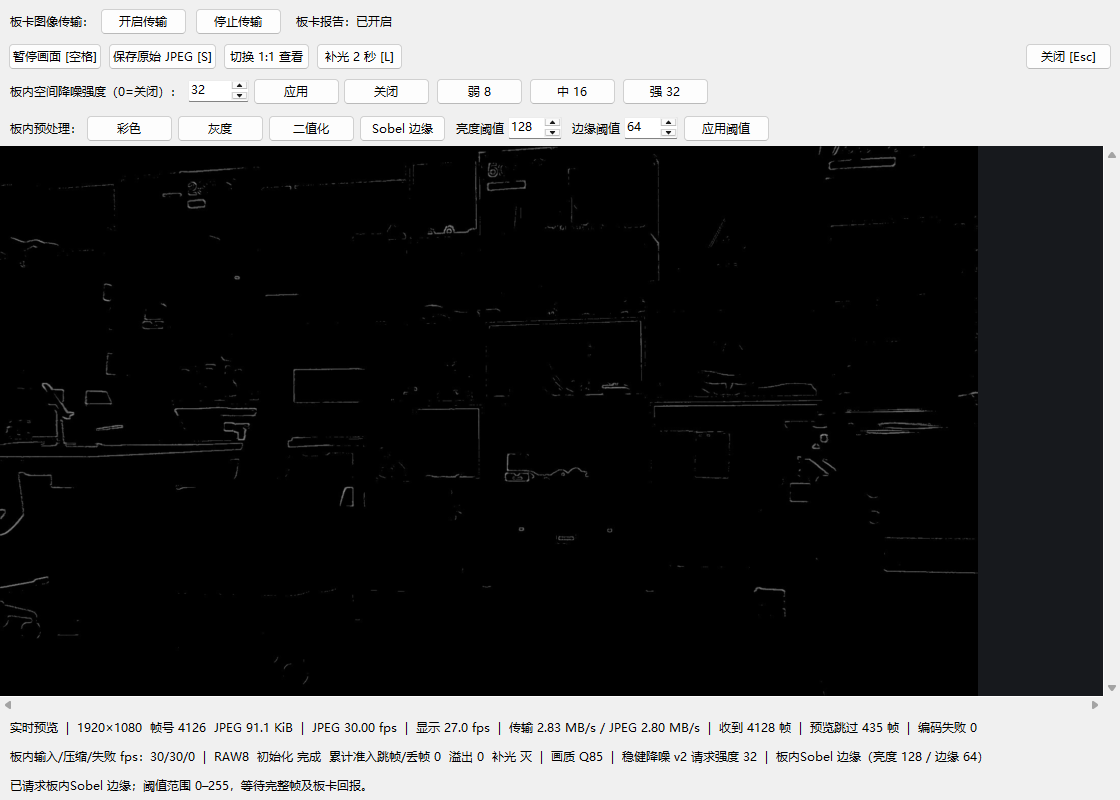
\includegraphics[width=.82\linewidth]{sobel_t064_window.png}
\caption{Sobel 边缘，$T_e=64$，Q85，N32。截图时 JPEG 91.1 KiB；稳定窗口 JPEG 载荷 2.80 MB/s、USB 接收 2.83 MB/s。}\label{fig:edge-64}
\end{figure}
\clearpage


\section{载荷、压缩效果与降噪观察}
\subsection{三档画质与本次实测带宽}
Q60、Q75、Q85 是本工程 JPEG 量化表的质量档位。较高 Q 通常保留更多量化后的细节，并增加 JPEG 大小；Q 值本身不是百分比压缩率。实际压缩比必须由原始有效载荷与压缩后的字节数计算，并注明原始格式。

本次在同一实验室场景、N32、彩色模式下依次测量三档画质，末尾再次测量 Q60，检查分时采集的场景漂移。每档切换后确认状态读回并等待稳定，采样约 12 s。下表使用十进制单位 $1\,\mathrm{kB}=1000$ B、$1\,\mathrm{MB}=10^6$ B；界面单帧大小使用 KiB，$1\,\mathrm{KiB}=1024$ B。

\begin{table}[H]\centering\caption{同场景 JPEG 质量与带宽实测}\label{tab:livequality}
\small\begin{tabular}{@{}lrrrrr@{}}\toprule
画质 & 样本帧数 & 均值 (kB/帧) & JPEG (MB/s) & USB (MB/s) & 压缩比\\\midrule
Q60 & 362 & 172.45 & 5.175 & 5.238 & 24.05:1\\
Q75 & 361 & 239.68 & 7.182 & 7.269 & 17.30:1\\
Q85 & 364 & 339.34 & 10.203 & 10.325 & 12.22:1\\
Q60 复测 & 363 & 172.27 & 5.178 & 5.241 & 24.07:1\\
\bottomrule\end{tabular}\end{table}

\begin{figure}[H]\centering
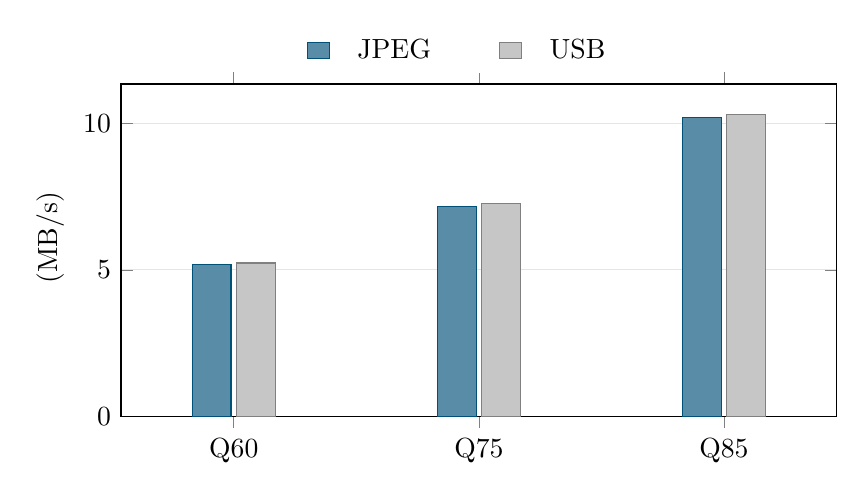
\begin{tikzpicture}
\begin{axis}[width=.88\linewidth,height=5.8cm,ybar,bar width=14pt,
 ymin=0,ylabel={带宽 (MB/s)},symbolic x coords={Q60,Q75,Q85},xtick=data,
 ymajorgrids=true,grid style={gray!20},legend style={at={(0.5,1.03)},anchor=south,legend columns=2,draw=none,column sep=8pt},
 legend image code/.code={\draw[#1] (0cm,-.1cm) rectangle (.28cm,.1cm);},
 enlarge x limits=.23]
\addplot[fill=teal!65,draw=teal] coordinates {(Q60,5.175) (Q75,7.182) (Q85,10.203)};
\addplot[fill=gray!45,draw=gray] coordinates {(Q60,5.238) (Q75,7.269) (Q85,10.325)};
\legend{JPEG 有效载荷,USB 接收记录}
\end{axis}\end{tikzpicture}
\caption{本次实测质量档位与带宽关系。帧率均约 30 fps，USB 读出记录包含 MBLK 开销。}\label{fig:livebandwidth}
\end{figure}
本次场景中，从 Q85 调低至 Q60，JPEG 平均载荷率从 10.203 MB/s 降至 5.175 MB/s，减少约 49.3\%。末尾 Q60 复测为 5.178 MB/s，相对首次变化 +0.04\%，用于提示分时统计的波动范围；不作为同输入压缩的严格误差界限。
\clearpage
\subsection{Q60 与 Q75 的界面带宽对照}
\begin{figure}[H]\centering
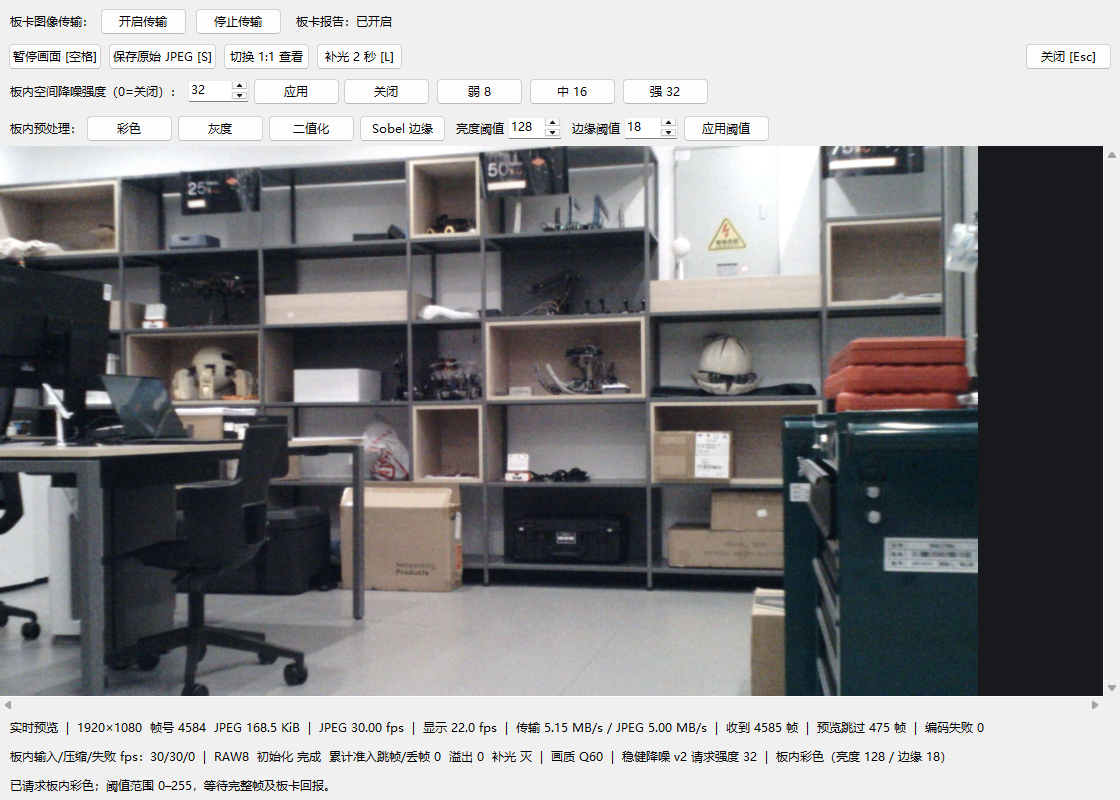
\includegraphics[width=.82\linewidth]{quality_q60_window.png}
\caption{彩色 Q60，N32。较低质量档位减少本场景的编码字节数。截图时 JPEG 168.5 KiB；稳定窗口 JPEG 载荷 5.18 MB/s、USB 接收 5.24 MB/s。}\label{fig:quality60}
\end{figure}
\begin{figure}[H]\centering
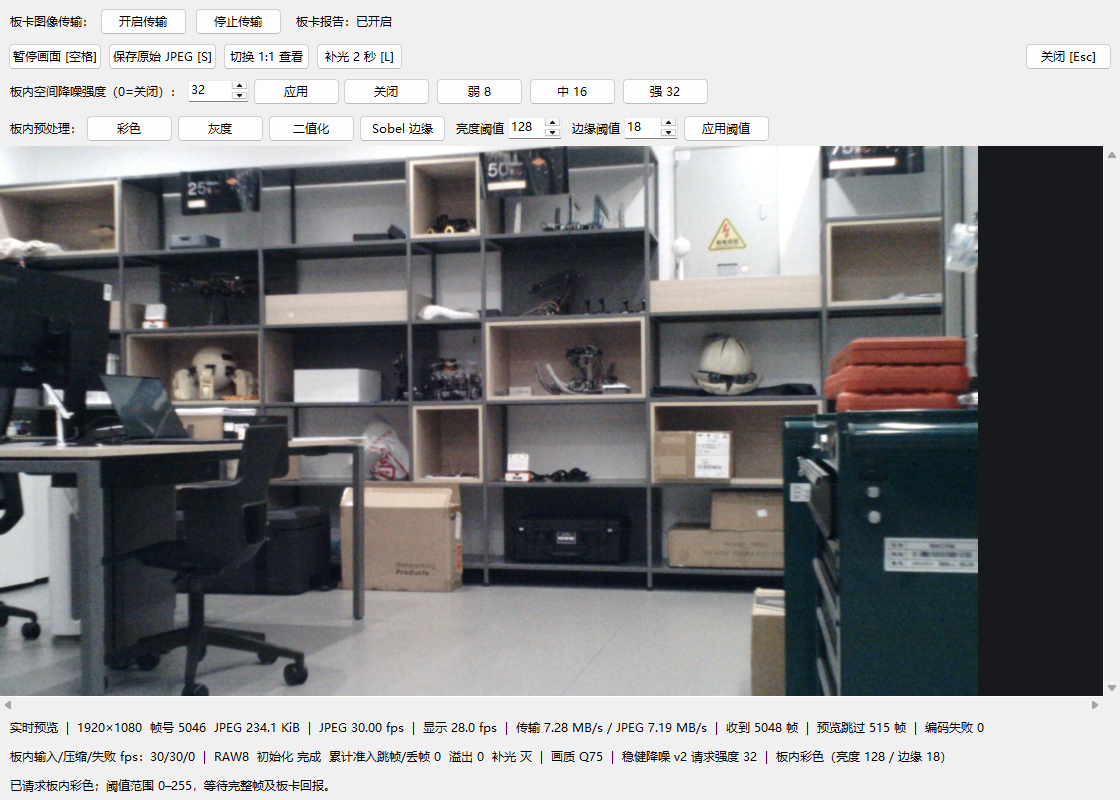
\includegraphics[width=.82\linewidth]{quality_q75_window.png}
\caption{彩色 Q75，N32。底部状态同时显示质量、帧大小、帧率和传输带宽。截图时 JPEG 234.1 KiB；稳定窗口 JPEG 载荷 7.18 MB/s、USB 接收 7.27 MB/s。}\label{fig:quality75}
\end{figure}
\clearpage
\subsection{Q85 与 Q60 复测的界面对照}
\begin{figure}[H]\centering
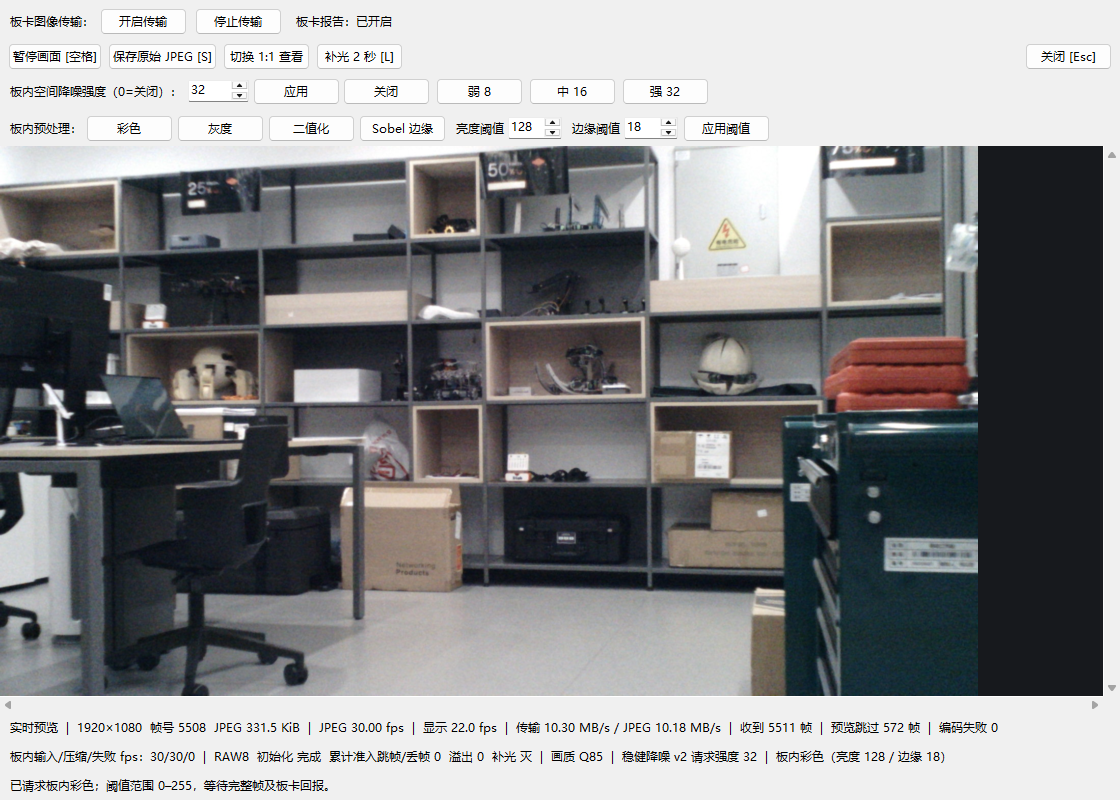
\includegraphics[width=.82\linewidth]{quality_q85_window.png}
\caption{彩色 Q85，N32。本次场景中载荷高于 Q60 和 Q75。截图时 JPEG 331.5 KiB；稳定窗口 JPEG 载荷 10.20 MB/s、USB 接收 10.32 MB/s。}\label{fig:quality85}
\end{figure}
\begin{figure}[H]\centering
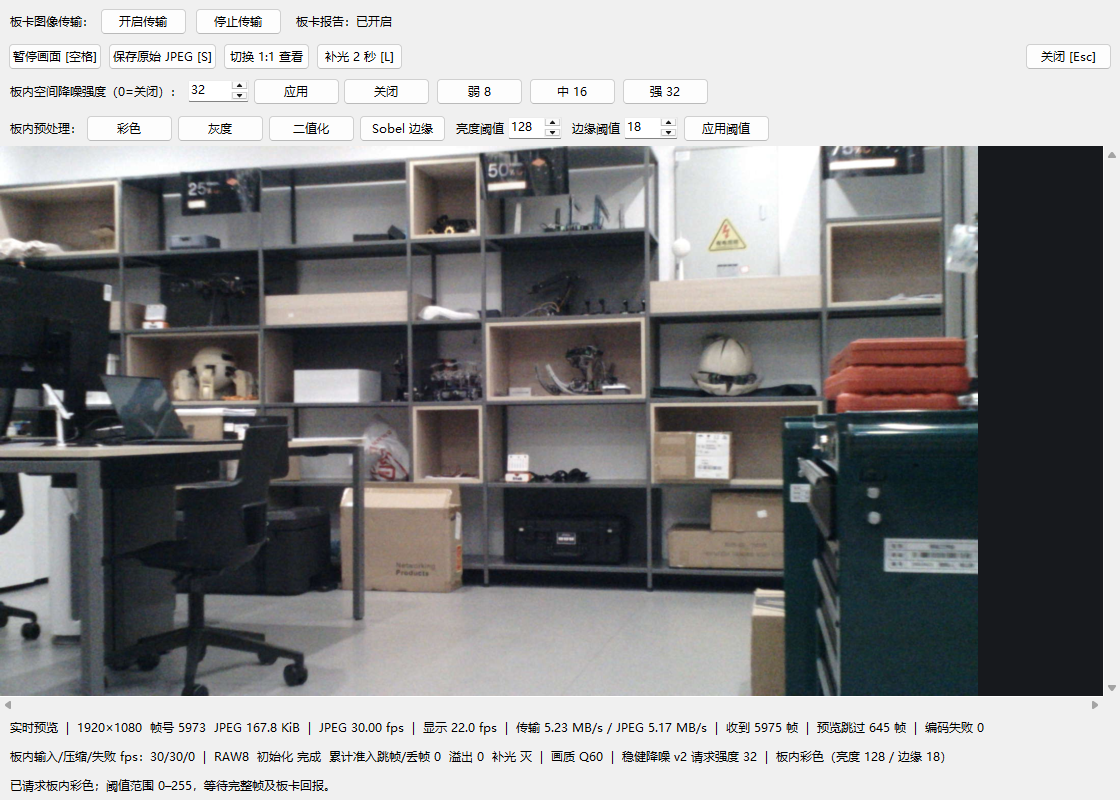
\includegraphics[width=.82\linewidth]{quality_q60_repeat_window.png}
\caption{返回彩色 Q60 复测，N32。检查本次分时采集的载荷漂移。截图时 JPEG 167.8 KiB；稳定窗口 JPEG 载荷 5.18 MB/s、USB 接收 5.24 MB/s。}\label{fig:quality60-repeat}
\end{figure}
\clearpage
\subsection{压缩比与带宽口径}
以编码前 YUV422 有效像素为参照，一帧大小为
\[
 S_{\rm YUV422}=1920\times1080\times2=4\,147\,200\ \mathrm{B},\qquad
 B_{\rm raw,30}=124.416\ \mathrm{MB/s}.
\]
设稳定窗口平均 JPEG 大小为 $\overline S_{\rm JPEG}$，则
\[
 R=\frac{4\,147\,200}{\overline S_{\rm JPEG}},\qquad
 \eta=\left(1-\frac{\overline S_{\rm JPEG}}{4\,147\,200}\right)\times100\%,\qquad
 B_{\rm JPEG}\approx\overline S_{\rm JPEG}\,f/10^6.
\]
Q60 的平均 JPEG 为 172445.76 B，按 YUV422 计算压缩比 24.05:1，有效载荷减少 95.84\%。Q75 的平均 JPEG 为 239675.46 B，按 YUV422 计算压缩比 17.30:1，有效载荷减少 94.22\%。Q85 的平均 JPEG 为 339341.77 B，按 YUV422 计算压缩比 12.22:1，有效载荷减少 91.82\%。

若改用传感器 RAW8 作为参照，一帧为 $2\,073\,600$ B，相应压缩比减半；两种基准不可混写。表\ref{tab:livequality}统一采用 YUV422。当前灰度、二值化和边缘仍沿用 JPEG 颜色帧及中性色度的链路格式，视觉上单色并不意味着传输变成无损 1 bit 像素流。

统计中的 JPEG 带宽为接收的完整 JPEG 字节增量除以主机单调时钟间隔；USB 带宽为相同窗口内解析器收到的 MBLK 记录字节增量，包含分块头、帧描述和状态记录。它不包含 USB 物理层握手、总线填充等全部开销，所以不能直接等同于 USB 总线利用率，也不能用标称 USB 2.0 速率直接反推链路余量。

本次 16 个稳定窗口的编码失败、FIFO 溢出及板内准入跳帧/丢帧增量均为 0，板卡时间戳计算的帧率约为 30.0019 fps。GUI 只解码显示选中的最新帧，本次采集未声明每个接收帧都经过独立完整像素解码；逐帧完整解码验收由前述严格接收器历史测试提供。截图不能单独替代长时间稳定性测试。
\evid{evidence/quality_q60.json；quality_q75.json；quality_q85.json；quality_q60_repeat.json}
\clearpage

\subsection{历史验收的载荷与降噪对照}
\begin{figure}[H]\centering
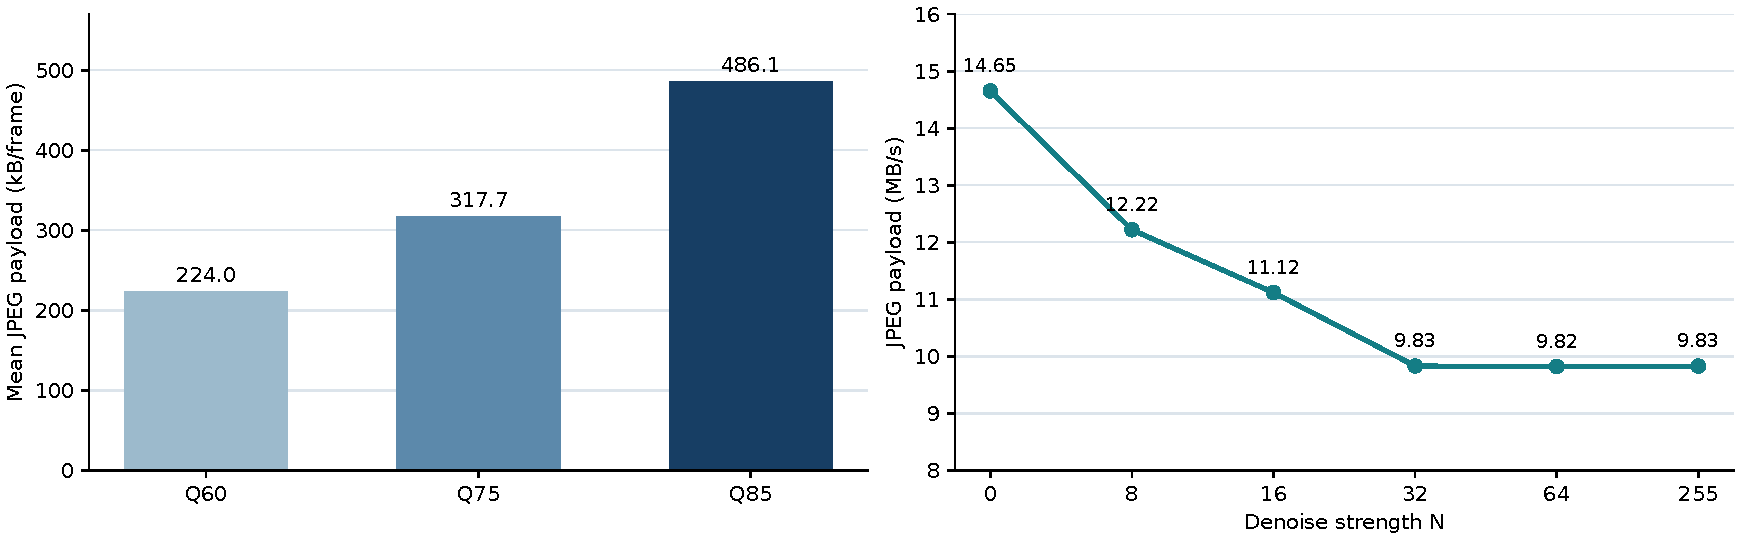
\includegraphics[width=.98\linewidth]{payload_results.pdf}
\caption{实板 JPEG 载荷。左图来自画质轮换，右图来自降噪重测前六段；均为分时实景统计。}\label{fig:payload}
\end{figure}
以下数据来自 2026 年 10 月 11 日的历史验收，场景和设置与本次演示不同。该次三档画质平均 JPEG 大小约为 224.0、317.7、486.1 kB/帧，帧率均约 30.002 fps。降噪重测中 N0 与 N32 载荷率分别约 14.654 MB/s、9.832 MB/s，下降约 32.9\%。抑制高频分量可以减小编码载荷，这种变化不能单独证明画质改善。

\begin{figure}[H]\centering
\begin{subfigure}{.485\linewidth}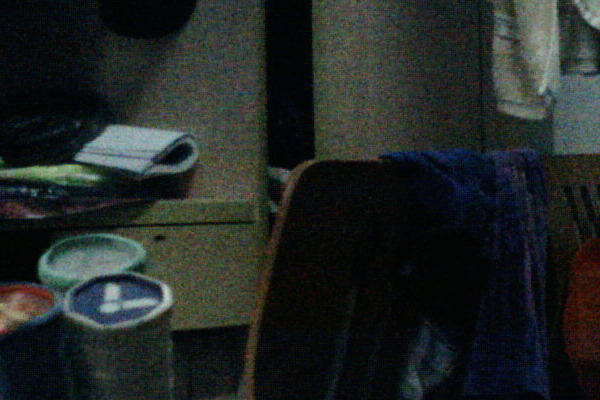
\includegraphics[width=\linewidth]{denoise_off_roi.png}\caption{N0：原样保留}\end{subfigure}\hfill
\begin{subfigure}{.485\linewidth}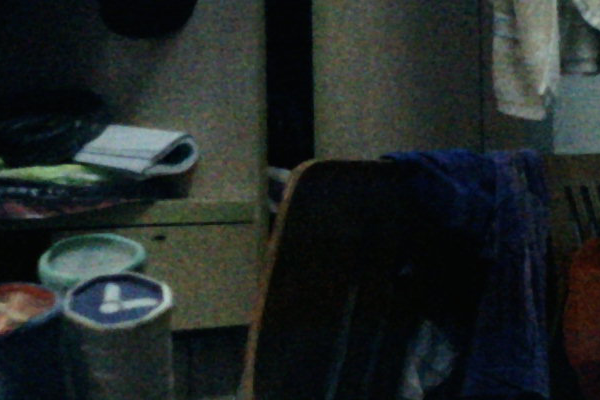
\includegraphics[width=\linewidth]{denoise_32_roi.png}\caption{N32：完整中值混合}\end{subfigure}
\caption{实拍局部对照，原图相同位置 $(500,400)$～$(1100,800)$ 裁剪，未锐化。分时采集，不作为相同输入下的定量画质比较。}\label{fig:nr}
\end{figure}
局部图中 N32 的墙面与织物色斑更平滑，部分纹理细节也可能减弱。当前缺少无噪声参考、曝光锁定和运动场景，不报告 PSNR、SSIM 或动态画质收益。

严格彩色长测使用 N32，平均 JPEG 为 326776.37 字节、约 9.804 MB/s。以 YUV422 有效载荷为基准，压缩比 12.69:1、载荷减少 92.12\%；以 RAW8 为基准则为 6.35:1、减少 84.24\%。不同原始格式必须标明计算基准，MBLK 和 USB 开销另计。
\clearpage

\section{总结与改进方向}
本项目实现了从 OV5640 RAW8 采集到 PC JPEG 解码显示的完整链路，在片上行缓存与 FIFO 结构下达到单路 1080p30 目标。设计将像素处理、独立 JPEG、同步 USB 和板卡控制组织为可验证模块，并通过描述符和计数器提供运行可观察性。

精简工作统一了最终源集合和工作流，移除退出链路的实验分支，再通过回归、重新构建与上板检验接口一致性。实板脚本残留命令的问题表明，维护范围应覆盖测试、文档和主机端。JPEG 核建立在已有移植基线上，后续工作包括链路集成、流控与资源时序优化；来源清单保存在仓库中，不能把全部基础核实现视为本次独立原创。

本次演示补充了四模式、二值化及 Sobel 多阈值和三档画质的真实窗口证据。阈值直接改变输出内容及载荷，画质档位则体现细节保留与传输带宽的取舍；所有比较均限定于当前分时采集场景。

后续优先改进三方面：其一，锁定曝光和白平衡，使用受控静态及运动场景评价色彩、暗光噪声和纹理；其二，针对摄像头输入与 USB 小裕量路径优化约束、布局并进行跨板、温压和长时间检查；其三，实测端到端显示时延，补齐物理按钮、灯光外观、复位和重连人工验收。现有结果支持当前配置下功能正常，不代替这些扩展评价。

\appendix
\section{构建、运行与复现}
在仓库根目录运行。需要 Vivado 2020.1、Python 3.10+、Pillow、NumPy 与 FTDI D2XX，同一时间只使用一个 USB 接收程序。
\begin{lstlisting}[language={},numbers=none,basicstyle=\fontsize{8.5}{10.5}\selectfont\ttfamily,caption={当前固件构建与验收命令}]
./mjpeg/scripts/run_camera_build.ps1 -Action Full
./mjpeg/scripts/run_camera_program.ps1 -Action Program
python mjpeg/host/camera_viewer.py
python -m unittest discover -s mjpeg/tb -p "test_*.py"
python mjpeg/host/camera_receiver.py --ftdi --duration 60 \
  --width 1920 --height 1080 --target-fps 30 \
  --require-fps 30 --require-no-drops --output <new_report_dir>
\end{lstlisting}
反斜杠仅表示排版续行；Windows PowerShell 中可合并为一行，或使用其续行语法。编译报告时在本目录执行两次 \texttt{xelatex main.tex}，生成目录与交叉引用。自包含源码和素材可复制到其他位置编译，不依赖仓库之外的本机绝对路径。
\clearpage

\section{版本、素材与证据索引}
实板验收基于提交 \texttt{d6549eb2d615814f57a4ce67899e98d9c6fead67} 的 RTL，主机降噪验收脚本随后修正旧命令探测。当前 bitstream 的 SHA-256 为：
\begin{quote}\small\ttfamily\nolinkurl{671ea1d5852a88fc94425ae3a3242bfe8885ffa734ed8a01d940b8d83ef3df1a}\end{quote}
LaTeX 工程保存源码节选、原图、完整原生截图及裁剪、数据摘要和素材 SHA-256。清单文件 \nolinkurl{asset_manifest.json} 记录原始路径与源码节选行号。以下证据按相对仓库路径定位：

\begin{table}[H]\centering\caption{关键证据索引}
\small\begin{tabularx}{\linewidth}{@{}p{37mm}Y@{}}\toprule
证据 & 相对路径或说明\\\midrule
精简回归 & \texttt{mjpeg/docs/}精简验证.json\\
当前完整构建 & \nolinkurl{mjpeg/reports/camera/full_20261011_123231/}\\
实板汇总 & \nolinkurl{mjpeg/reports/camera/cleanup_acceptance_20261011_124020/hardware_summary.json}\\
原生数据库 & \nolinkurl{mjpeg/reports/camera/waveforms_20261025/camera.wdb}，同目录 \texttt{controls.wdb}\\
本次演示截图与统计 & \nolinkurl{mjpeg/reports/camera/report_demo_20261026/summary.json}，同目录 \texttt{*\_window.png} 与分段 JSON\\
原生截图与配置 & 同目录 \texttt{vivado\_*.png} 与 \texttt{*native*.wcfg}\\
源码来源 & \nolinkurl{mjpeg/docs/copied_rtl_manifest.json}；\nolinkurl{mjpeg/docs/original_source_snapshot.json}\\\bottomrule
\end{tabularx}\end{table}

\begin{thebibliography}{9}\small\raggedright
\bibitem{jpeg} ITU-T. Recommendation T.81: Digital compression and coding of continuous-tone still images -- Requirements and guidelines[S]. 1992. \url{https://www.itu.int/itu-t/recommendations/rec.aspx?id=2633&lang=en}.
\bibitem{ftdi} FTDI. FT232H Single Channel Hi-Speed USB to Multipurpose UART/FIFO IC Datasheet[EB/OL]. \url{https://ftdichip.com/wp-content/uploads/2020/07/DS_FT232H.pdf}.
\bibitem{ug900} Xilinx. Vivado Design Suite User Guide: Logic Simulation, UG900, v2020.1[EB/OL]. \url{https://docs.amd.com/v/u/2020.1-English/ug900-vivado-logic-simulation}.
\bibitem{project} MotionJPEG 项目. 当前 RTL、接口文档、原始仿真输出与实板验收记录[Z]. 本地资料，2026 年 10 月整理。在线资料访问日期：2026-10-25。
\end{thebibliography}

\end{document}
